\chapter{意识障碍}

意识障碍是指人对周围环境及自身状态的识别和觉察能力出现障碍。多由高级神经功能受损所致,根据意识水平和意识内容损害程度不同分为嗜睡、意识蒙眬、意识模糊、谵妄、昏睡、昏迷(轻度、中度、重度)。

\section{【发生机制】}

人的意识活动由意识内容及其“开关”系统两部分组成。意识活动包括记忆、思维、定向、情感等精神活动,以及通过视、听、语言和复杂运动等与外界环境保持紧密联系的能力。“开关”系统包括特异性上行投射系统(各种感觉传导通路的总称),以及非特异性上行投射系统(上行性网状激活系统和上行性抑制系统)。上行性网状激活系统位于脑桥下1/3到间脑中央部中线两旁、脑室的腹侧。它接受特异性上行投射系统的侧支纤维的激活,由此再产生兴奋冲动经丘脑的非特异性核如板内核、中继核、腹前核等,弥散地作用于整个大脑皮质,从而使大脑维持觉醒状态。另一方面,意识活动也取决于大脑半球的完整性。正常时,大脑半球接受特异性上行投射系统和非特异性上行投射系统的激活,它也发出兴奋冲动到脑干网状结构。因而人觉醒状态的维持,有赖于上行性网状激活系统和大脑皮质的正常功能及其相互作用。颅内、外各种病变若累及上行性网状激活系统的任何一个环节,即可引起意识障碍。例如脑干的出血、梗死、占位病变、炎症等,因直接累及上行性网状激活系统而导致严重的意识障碍。大脑半球局限性病变不会引起意识障碍,只有相当广泛而严重的病损才会引起意识障碍。例如,大脑半球的占位性病变或血管性疾病导致颅内压增高,产生脑疝,压迫间脑和中脑上部上行性网状激活系统而致昏迷。代谢性疾病、内分泌疾病或其他全身性疾病最终波及脑干网状结构,使网状结构神经元突触后膜对递质的敏感性极度降低,突触传递停止或是神经递质的合成停止,导致患者出现意识障碍。

\section{【意识障碍的分类】}

临床上根据意识水平损害的轻重将意识障碍分为嗜睡、昏睡、昏迷;根据意识内容损害的程度又可将意识障碍分为意识蒙眬、意识模糊和谵妄。

\subsection{(一)嗜睡}

嗜睡是最轻的意识障碍,呈现病理性倦睡,可被唤醒正确回答问题并做出相应的反应,对时间、空间和人物的定向力正常,停止刺激后患者又进入睡眠状态。

\subsection{(二)昏睡}

昏睡是较严重的意识障碍,患者需经过强烈和连续的刺激(持续压眶刺激)才能唤醒,唤醒后反应迟钝,时间、空间定向力障碍,无法正常交流,一旦停止刺激立即进入睡眠状态。

\subsection{(三)昏迷}

昏迷是最严重的意识障碍,表现对周围事物和声光刺激丧失反应,意识活动完全中断和丧失,根据程度不同分为轻度、中度和重度。

\subsubsection{1.轻度昏迷}

也称浅昏迷或半昏迷:患者的随意运动丧失,对周围事物以及声、光等刺激全无反应,但在强烈的疼痛刺激时(如压迫眶上神经)可见患者有痛苦表情、呻吟和下肢的防御反应;吞咽反射、咳嗽反射、角膜反射以及瞳孔对光反射仍然存在;呼吸、脉搏、血压一般无明显改变。大、小便潴留或失禁。

\subsubsection{2.中度昏迷}

患者对周围事物及各种刺激均无反应,对于剧烈的刺激或可出现防御反应;角膜反射减弱,瞳孔对光反射迟钝,眼球无转动。呼吸、脉搏、血压已有改变;大、小便潴留或失禁。

\subsubsection{3.重度昏迷}

全身肌肉松弛,对各种刺激全无反应。腱反射、吞咽反射、咳嗽反射、角膜反射和瞳孔对光反射均消失。呼吸不规则,血压或有下降,大、小便失禁,偶尔潴留。此时机体仅能维持最基本的功能。

\subsection{(四)意识蒙眬}

意识范围的缩小,可感知事物的轮廓,但不清晰;定向力下降,清醒后回忆不完整。

\subsection{(五)意识模糊}

意识活动存在,但对时间、地点、人物等定向力障碍。

\subsection{(六)谵妄}

患者在意识模糊的基础上同时出现了幻觉和妄想(多见于感染性疾病高热期和中毒性脑病)。

意识障碍疾病的分类(表\ref{tab49-1})

\begin{longtable}{c}
 \caption{意识障碍疾病的分类}
 \label{tab49-1}
 \endfirsthead
 \caption[]{意识障碍疾病的分类}
 \endhead
 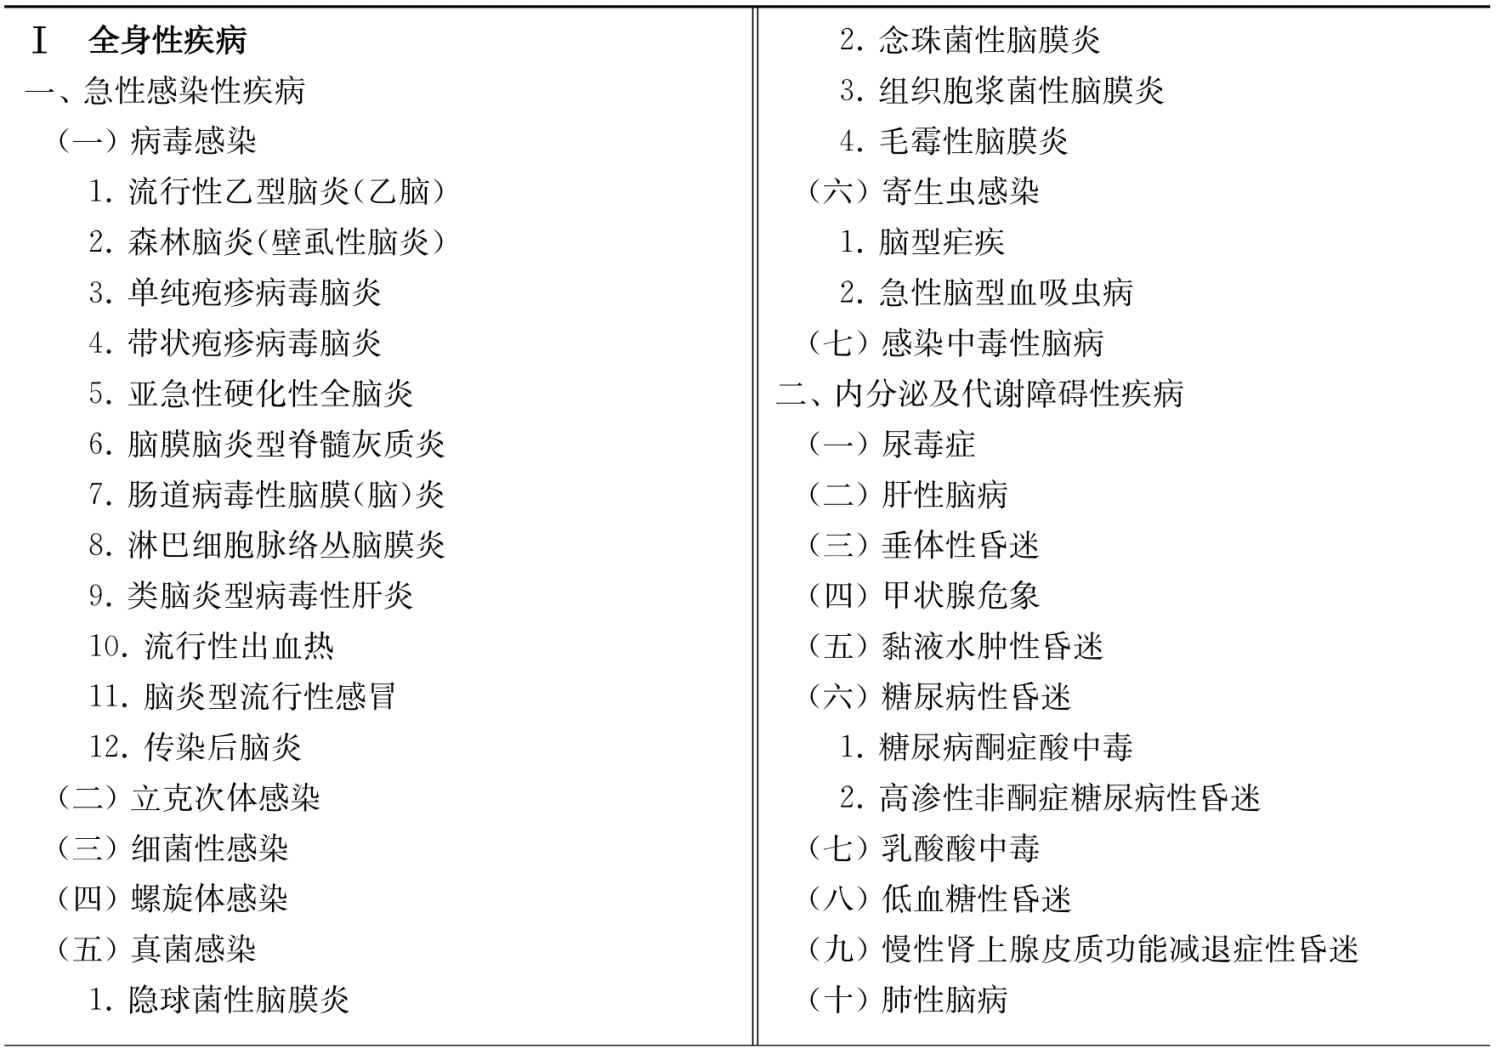
\includegraphics[width=\textwidth,height=\textheight,keepaspectratio]{./images/Image00305.jpg}\\
 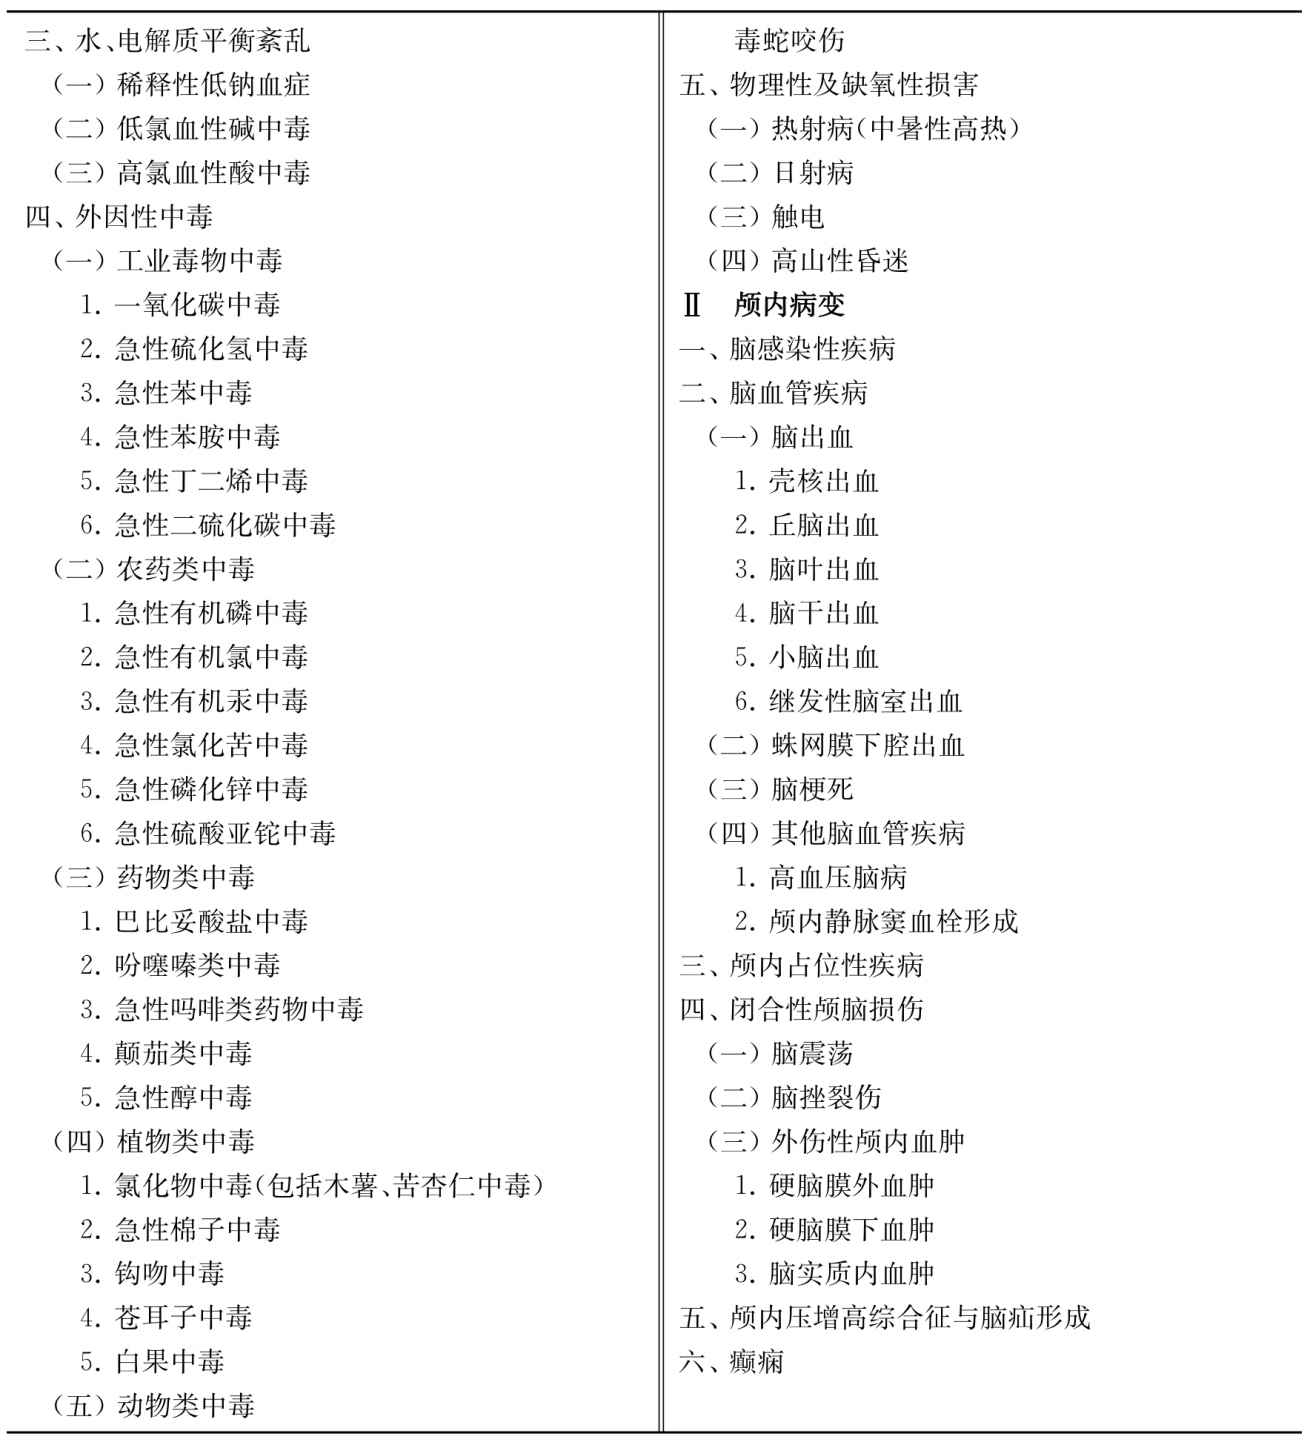
\includegraphics[width=\textwidth,height=\textheight,keepaspectratio]{./images/Image00306.jpg}
 \end{longtable}

\section{【意识障碍的鉴别】}

意识障碍需与下列几种貌似意识障碍的状态鉴别:

\subsection{(一)去皮质状态}

大脑两侧皮质发生弥散性的严重损害引起皮层功能丧失,而皮层下结构的功能仍保存或部分恢复,形成意识丧失、肢体强直等。临床表现为患者常瞪眼凝视(也称瞪目昏迷或醒状昏迷),能无意识地睁、闭眼,眼球能活动,瞳孔对光反射、角膜反射存在,四肢肌张力增高,双上肢屈曲,双下肢伸直,病理反射阳性。可有吸吮反射、强握反射。甚至喂食也可以引起吞咽,但无自发动作,对外界刺激不能产生有意识的反应,大、小便失禁,存在睡眠-觉醒周期。

\subsection{(二)无动性缄默症}

是由于脑干或丘脑上行性网状激活系统的不完全性损害所致,而大脑半球及其传出通路则无病变。患者不言、不语、不动,意识内容丧失,四肢肌张力增高,但无锥体束征,吞咽等反射活动保留,瞬间反射存在,对疼痛刺激有躲避反应,存在睡眠-觉醒周期。

\subsection{(三)持续植物状态}

主要为前脑结构,尤其大脑皮层的广泛损害。基本表现为睁眼昏迷,存在睡眠觉醒周期,但无任何意识心理活动,保存吸吮、咀嚼、吞咽等原始反射。对有害刺激可有肢体屈曲躲避反应,大、小便失禁。

\subsection{(四)闭锁综合征}

是由于脑桥腹侧的局限性病变累及双侧皮质脊髓束,以及三叉神经以下的皮质延髓束所致。患者能睁、闭眼,眼球能垂直运动而不能水平运动。因上行性网状激活系统未受累之故,患者的意识活动存在,能以眼球的上、下活动来表达其思维活动。本综合征的常见病因是基底动脉主干闭塞,偶见于脑桥出血、肿瘤和脑桥中央髓鞘溶解症,神经影像学和脑血管学检查有助于诊断。

\subsection{(五)紧张综合征}

包括木僵、违拗、刻板言语和动作、模仿言语和动作、蜡样屈曲、缄默等症状,可以持续数周至数月。紧张性木僵可以突然转入紧张性兴奋状态。紧张性兴奋持续时间短暂,常常是突然暴发的兴奋和暴力行为,然后又突然进入木僵或缓解。典型的紧张综合征见于精神分裂症的紧张型,其他精神病、抑郁症、反应性精神障碍、颅脑损伤时也可见到不典型的表现。

\subsection{(六)晕厥}

是由多种原因导致一过性脑供血不足而发生短暂的意识丧失,常见类型为血管迷走性晕厥、心源性晕厥和脑源性晕厥。昏迷与晕厥的鉴别要点是前者的意识丧失时间较长,不易迅速逆转;后者则是为短暂的意识丧失。

\subsection{(七)发作性睡病}

为一组睡眠障碍性疾病,典型表现为四联症,分别是不可抗拒的病理性睡眠、猝倒发作、入睡前睡眠幻觉、睡眠瘫痪。发作性睡病与昏迷不同,前者是睡眠障碍,患者在正常人不易入睡的场合下,如行走、骑自行车、工作、进食时均能出现难以控制的睡眠,其性质与生理性睡眠无异,持续数分钟至数小时,但可唤醒。

\subsection{(八)癔症}

是临床上常见的一类精神心理障碍性疾病,发作时需要与意识障碍之昏迷相鉴别,癔症的意识障碍仅为意识范围的缩窄而非意识丧失。患者在发作时仍有情感反应(如眼角噙泪)以及主动抗拒(在扒开患者的双眼时患者的眼睛反而闭合更紧,称之违拗)等。

\subsection{(九)阵发性意识障碍}

某些意识障碍呈阵发性出现,称为阵发性意识障碍。这种情况可见于肝硬化、胰岛细胞瘤、脑部中线肿瘤。偶有阵发性昏迷并伴有阵发性精神症状的患者,需考虑间脑病变的可能。

了解意识障碍发生的全过程,对意识障碍的鉴别诊断有重要意义。意识障碍发生急骤并成为疾病的首发病征者,常见于颅脑损伤、脑血管疾病、外源性中毒、热射病、日射病,以及某些中枢神经系统急性感染,如暴发型流行性脑膜炎;在疾病发展过程中较为缓慢发生的意识障碍,可见于代谢障碍疾病,如肝性脑病和尿毒症性昏迷、脑肿瘤和结缔组织病等。

急性颅内或颅外感染性疾病所致的意识障碍,其基本规律是意识障碍前先有发热。发病于冬春者多见于流行性脑膜炎、斑疹伤寒、回归热、大叶性肺炎等;发病于夏秋者多见于乙型脑炎、脑干型脊髓灰质炎、脑型疟疾、中毒型菌痢、伤寒等。在高温或烈日下工作而突然意识障碍者,多考虑热射病和日射病。意识障碍前经常有头痛或伴以呕吐者,应考虑颅内占位性病变的可能。患有高血压动脉硬化的老年人突然发生意识障碍时,应首先想及脑血管疾病。颅脑损伤后昏迷时间的长短以及有无中间清醒期,可协助诊断有无继发性颅内血肿,甚至有助于提示硬脑膜外或硬脑膜下血肿。

\section{【诊断思路】}

病史中尤应注意既往有无高血压、动脉硬化、糖尿病、心脏病、肝脏病、肾脏病、癫痫等情况。昏迷前的用药史也有助于鉴别诊断,如使用过量胰岛素所致的低血糖性昏迷,慢性肝脏病患者因应用氯丙嗪或巴比妥类药物而诱发的肝性脑病。

体格检查对意识障碍的鉴别往往能提供若干线索。下列各项内容需要细致的观察:

\subsection{(一)皮肤}

皮肤灼热、干燥见于热射病昏迷;皮肤湿润见于低血糖性昏迷、吗啡类药物中毒、心肌梗死和日射病等;皮肤苍白见于尿毒症性、低血糖性昏迷等;皮肤潮红见于脑出血、颠茄类中毒及酒精中毒;一氧化碳中毒的口唇常为樱红色;肝性脑病患者的皮肤多伴黄疸;唇颊和手指发绀以及静脉充盈,提示心脏功能不全或肺功能不全所致的缺氧;单纯的发绀见于某些化学物品中毒。皮肤见有出血点,应警惕流行性脑脊髓膜炎;皮肤出现蔷薇疹者提示伤寒的可能;口唇疱疹可并发于大叶性肺叶、流行性脑膜炎、间日疟等疾病。此外,尚需检查皮肤尤其是头颅部分皮肤有无伤痕或骨折,可以作为颅脑损伤以及癫痫大发作的佐证。

\subsection{(二)呼吸}

呈深大呼吸者应考虑代谢性酸中毒(糖尿病、尿毒症等);鼾声呼吸且伴有呼吸时一侧面肌瘫痪者提示脑出血;呼吸急促多为急性感染性疾病;低血糖性昏迷的呼吸则较浅。呼气带有氨味见于尿毒症性昏迷;呼吸带有烂苹果味见于糖尿病性昏迷;若杏仁气息提示氢氰酸(苦杏仁、木薯、氰化物等)中毒;呼气及排泄物(尤其是尿液)有大蒜样臭味者可见于有机磷农药中毒;呼气中及尿液出现“肝臭”者提示为肝性脑病。

脑部不同水平损害可引起不同的呼吸紊乱形式,这有助于病变水平的定位。例如,脑部广泛损害或代谢障碍时,可引起过度换气后呼吸暂停现象;双侧大脑深部病变或天幕上占位病变,可产生潮式呼吸;中脑下部和脑桥上部病变,可引起中枢神经性过度换气;脑桥下部病变,可引起长吸式呼吸;Biot呼吸(呼吸深浅或节律完全不规则)见于延髓背内侧病变,表示病情危笃。

\subsection{(三)发热}

意识障碍伴发热常见于各种颅内外感染、脑出血或蛛网膜下腔出血;昏迷伴体温过低可见于休克、低血糖、中毒、甲状腺功能减退、肾上腺皮质功能减退等。

\subsection{(四)脉搏}

脉搏触诊有助于及时发现阿司综合征。脉慢而充盈见于脑出血、酒精中毒;脉慢而弱见于吗啡类药物中毒;脑脓肿患者的脉搏常缓慢、充实而规则,而脑膜炎患者的脉搏多细速。颠茄类中毒、氯丙嗪中毒时脉搏显著加快。

\subsection{(五)眼症状}

昏迷患者的眼球活动异常或眼球位置异常,可提示脑部受损的平面。例如,患者不能眨眼,说明脑干网状结构已受抑制。患者若有自发性眼球浮动(以水平性多见),说明昏迷的程度较浅,脑干功能仍存在。当中脑或脑桥损害时,眼球浮动消失而固定于中央位置。眼球沉浮(两眼迅速向下方偏转,超过正常俯视的范围,而后缓慢向上回到正常的位置),可见于脑桥局限性病变。眼激动(不安眼)常见于两侧大脑半球损害,如两侧卒中、脑炎、肝性脑病。双眼向下偏视(凝视鼻尖),见于丘脑或丘脑底部病变、中脑广泛病变。两眼向偏瘫对侧注视时,提示病灶在大脑半球;两眼向偏瘫侧注视时,提示病灶在脑干。明显的分离性斜视,表示中脑受累或动眼神经瘫痪。垂直性分离性斜视,意味着颅后窝损害。昏迷患者有完整的两眼反射性水平协同运动时,提示病变仍限于大脑半球,若病变累及脑干则此种运动消失。将患者的头部向两侧及前、后轻轻但较快地移动,可见两眼球协同向相反的方向转动,称为玩偶眼现象,提示昏迷较浅;倘若脑干广泛损害或巴比妥类药物中毒,则此征象消失。瞳孔改变是意识障碍患者一项极为重要的体征,常能提示某些病因及反映病情的变化。双侧瞳孔散大可见于多种药物或食物中毒,如颠茄类、巴比妥类(有时瞳孔缩小)、可待因、氰化物、肉毒杆菌中毒等;双侧瞳孔缩小见于氯丙嗪、吗啡类药物、有机磷、水合氯醛、毒蕈等中毒与尿毒症。双侧瞳孔缩小如针眼、伴有高热是原发性脑桥出血的特征,若患者还有四肢阵发性强直性抽搐,则是脑室出血的表现。两侧瞳孔大小不等或忽大忽小,可能是脑疝的早期征象;一侧瞳孔散大和对光反射消失,是蛛网膜下腔出血、颅内血肿以及小脑幕切迹疝等病变压迫动眼神经的结果。双侧眼球同向偏斜的急性昏迷患者,提示有脑出血或大面积脑梗死的可能;突然昏迷而伴有单侧眼肌麻痹的患者,有可能是脑动脉瘤破裂出血;昏迷患者伴有高热和一侧(有时是双侧)眼球突出以及眼外肌麻痹时,要想到海绵窦血栓性静脉炎。

对昏迷患者进行眼底检查,其重要性自不待言。视乳头水肿是颅内压增高重要而客观的指征;视网膜有渗出、出血以及动脉改变,有助于尿毒症、恶性高血压和糖尿病的诊断。玻璃体下出血常见于蛛网膜下腔出血。

\subsection{(六)颈项强直}

颈项强直是各种脑膜炎和蛛网膜下腔出血常见而有诊断意义的征象,颈项强直或伴有颈痛应警惕早期枕骨大孔疝的可能。

\subsection{(七)神经系统局灶体征}

昏迷患者有无神经系统局灶体征,有助于鉴别是全身性病变所致的昏迷抑或颅内病变所致的昏迷。如伴有偏瘫体征,则提示颅内有局灶性神经系统病变,常见于脑血管病、脑部感染、颅脑损伤、颅内占位性病变等。但无局灶性神经系统病征的昏迷也可能是颅内病变,例如蛛网膜下腔出血、脑积水或脑内静脉窦血栓形成,不少患者除颈项强直之外,并未发现神经系统的局灶体征,如癫痫发作后的昏迷,局灶性神经系统病征常缺如。发生昏迷的某些化脓性脑膜炎患者不一定伴有脑膜刺激征,尤其是婴幼儿或老年患者在疾病的早期阶段。昏迷患者伴有双侧巴宾斯基征阳性,见于多种原因所致的昏迷,如脑血管病、颅脑损伤、颅内感染、低血糖状态和中毒性昏迷等。

\subsection{(八)不随意运动}

意识障碍伴有不随意运动如肌肉抽搐见于尿毒症、肺性脑病;扑翼样震颤多见于肝性脑病,也可见于肺性脑病;二硫化碳、阿托品类、有机氯等中毒可发生阵发性抽搐;一氧化碳、有机磷、氰化物、士的宁等中毒可引起强直性抽搐;使用胰岛素过量可引起阵发性或强直性抽搐;癫痫样发作可见于高血压脑病、脑出血、蛛网膜下腔出血、脑栓塞、颅脑损伤等疾病;舞蹈样动作见于风湿性脑病。

\subsection{(九)伴有精神症状的意识障碍}

如谵妄多由于感染、蛛网膜下腔出血或外源性中毒所引起;昏迷而有兴奋躁动,见于颅脑损伤、酒精中毒等;昏迷患者显得安静,所谓宁静型昏迷,见于尿毒症、营养不良或衰竭性昏迷等。

\subsection{(十)其他}

浅昏迷患者出现频频的呃逆或呵欠,表示颅内压增高;呃逆有时也可见于尿毒症性昏迷前期。

上述各种体征有些虽有特异性,但切勿根据一种征象而下诊断,临床医生必须结合其他检查结果全面考虑,方能作出较为正确的诊断。

实验室检查对昏迷有一定的诊断价值,可根据初步的临床印象选择有关的检查。

本章按表\ref{tab49-1}的顺序分别讨论。

\protect\hypertarget{text00370.html}{}{}

\section{163 全身性疾病}

\subsection{163.1 急性感染性疾病}

\subsubsection{163.1.1 病毒感染}

\paragraph{一、流行性乙型脑炎(乙脑)}

乙脑患者约2/3有意识障碍,自轻度倦睡乃至深度昏迷。凡在夏秋季节,在乙脑病区,有蚊虫叮咬史,尤其是儿童与青年人,突然高热兼有惊厥、意识障碍等神经精神症状时,应考虑乙脑的可能性。

患者通常急骤起病,在2~3天内多有嗜睡、昏睡或昏迷;或初有谵妄、惊厥而后转入昏迷。发热是常见的症状,常达40℃或以上。发热的高低常与神经系统症状的轻重成正比。如患者昏迷程度深,惊厥严重而体温不高,或仅轻微发热,则乙脑的可能性甚少。如昏迷先于发热或高热起病而立即昏迷者,也不符合乙脑症状。脑膜刺激征见于70\%~80\%的病例,脑脊液符合病毒性感染的改变。血象白细胞增多(常达10~20×10\textsuperscript{9}
/L),分类中性粒细胞增多与核左移,对除外其他病毒性脑膜脑炎可有参考价值。

神经系统症状多在病后1~2周内达到最高峰;如在2周后才出现昏迷,则应考虑其他疾病。患者的大脑皮质症状也较其他中枢神经症状为重,如有肢体瘫痪也必有意识障碍,若急性期有肢体瘫痪而意识清楚,则大致可除外乙脑。

有的中毒型菌痢患者在腹泻未出现前先有高热、惊厥与昏迷,每易误诊为乙脑。前者通常有进食不洁饮食史,早期出现休克,一般无脑膜刺激征,肛检或盐水灌肠常能发现脓血或黏液便,脑脊液符合化脓性炎症改变。有时肺炎或败血症早期所致的中毒性脑膜脑炎(尤其是腮腺炎病毒及肠道所引起者)在临床上均可与乙脑类似,需细心加以鉴别。

乙脑的确诊有赖于流行病学史、上述临床表现及血清补体结合试验,但后者对早期诊断帮助不大。阳性率于病后1~2周逐渐增加,在第4周以后达60\%~80\%。通常于病程第1周以及第3或4周后各测定一次,如第二次的滴度较第一次增加四倍,则为阳性。若只有急性期单份血清标本,滴度在1∶2时为可疑,1∶4为阳性。

\paragraph{二、森林脑炎(壁虱性脑炎)}

诊断森林脑炎必须注意流行病学史。森林脑炎是森林地区特有的急性传染病,有严格的地域性与季节性。在某些地区发生于5~8月。患者主要为从事林业的人,发病年龄以20~40岁居多,尤以新近进入该病区的人常见。一般均有被壁虱叮咬史。凡患者急性高热、意识障碍、颈、肩肌及肢体瘫痪而兼有上述流行病学史者,需考虑森林脑炎的可能性。

本病潜伏期为10~15天。患者通常突然发病,呈高热或过高热、头痛、恶心、呕吐、意识不清、昏睡或昏迷,并迅速出现脑膜刺激征。昏睡与瘫痪是本病的主要特征,对诊断有意义。患者常于发病后2~5天迅速出现颈肌、肩胛肌与肢体瘫痪,多累及上肢,其次为下肢或上下肢。此种瘫痪与乙型脑炎不同,呈弛缓性,故有鉴别诊断意义。血象白细胞增多,分类计数中性粒细胞增多。脑脊液压力正常或稍高,无色透明,蛋白量轻度增加,糖与氯化物均正常,细胞数多在50~200×10\textsuperscript{6}
/L之间,分类以淋巴细胞占优势。确诊需依靠特殊的补体结合试验或病毒分离。

森林脑炎容易与脊髓灰质炎相混淆,流行病学史是重要的区别点之一,且脊髓灰质炎少有意识障碍,血清学检查是主要的鉴别根据。此外,也需注意与乙型脑炎相鉴别,主要根据脑脊液中特异性抗体的存在。

\paragraph{三、单纯疱疹病毒脑炎}

单纯疱疹病毒脑炎又称急性坏死性脑炎或出血性脑炎。是由单纯疱疹病毒引起的中枢神经系统最常见的病毒感染性疾病。意识障碍是常见症状,早期以嗜睡多见,随病情进展意识障碍加重,最后昏迷。

单纯疱疹病毒是一种嗜神经DNA病毒,经呼吸道感染隐藏于三叉神经节,数年后或机体免疫力低下时,非特异性刺激可诱发病毒激活而发病。国外报道发病率为(4~8)/10万,患病率为10/10万。病理改变为颞叶、额叶等部位出血性坏死、脑水肿。

任何年龄均可患病,无地区性和季节性。急性起病,初有发热、全身不适、头痛、肌痛、嗜睡、腹痛和腹泻等前驱症状,约1/4的患者有口唇疱疹病史。发病时中至高度发热,精神异常、人格改变是本病的突出表现,个别病例以全身性或部分性运动性发作为首发症状,意识障碍多伴随于精神异常,并随病情进展而加重,最后昏迷。神经症状可有偏盲、偏瘫、失语、眼肌麻痹、多动、脑膜刺激征等弥散性和局灶性脑损害的表现。重症患者可因广泛脑实质坏死和脑水肿引起颅高压,甚至脑疝形成。病程为数日至1~2个月,死亡率高,有后遗症。

脑电图可见弥漫性高波幅慢波;头颅CT可见一侧或双侧颞叶、海马及边缘系统局灶性低密度区,若低密度灶中出现点状高密度影提示颞叶有出血,更支持本病的诊断,头颅MRI检查有助于诊断;脑脊液压力正常或轻度增高,细胞数明显增多,以单个核细胞为主,可有红细胞增多,蛋白质轻中度增高,糖和氯化物正常。

诊断依据疱疹病史、发热、明显的精神行为异常、抽搐、意识障碍,以及脑脊液、脑电图、脑CT改变,特异性抗病毒治疗有效可间接支持诊断。注意与带状疱疹病毒脑炎、肠道病毒脑炎、巨细胞病毒脑炎及急性播散性脑脊髓炎相鉴别。

\paragraph{四、带状疱疹病毒脑炎}

意识障碍是带状疱疹病毒脑炎的常见症状,多数患者表现为昏睡,少数病例可发展为昏迷甚至死亡。

带状疱疹病毒与水痘病毒一样,属脱氧核糖核酸疱疹病毒,初次感染常发生于儿童,病毒感染后可长期潜伏于脊神经节细胞内或三叉神经节细胞内。当各种原因导致机体免疫功能低下时,潜伏的病毒可被激活复制,并在相应的感觉神经节段皮肤出现带状或束状疱疹,亦可沿感觉神经上行入脑,数周后发生脑炎或脑膜炎。临床表现为突然发热、头痛、呕吐、抽搐、偏瘫、失语、精神异常及意识障碍,部分患者可有脑神经损害、共济失调或脑膜刺激征。一般病情较轻,常见于中年患者,多数经治疗数周或数月痊愈。少数开始表现为躁狂、谵妄,继而昏睡、昏迷甚至死亡。脑脊液白细胞轻至中度增高(最高达500个/mm\textsuperscript{3}
),蛋白质可正常或轻至中度增高,糖与氯化物正常。补体结合试验可显示带状疱疹病毒抗体阳性。皮疹明显者,皮肤受损细胞活检可查到核内包涵体。头颅CT及MRI扫描显示带状疱疹同侧大脑中动脉区内,包括内囊及大脑皮层、皮层下椭圆形、边界清楚的多灶性梗死灶,颈动脉造影可见大脑中动脉近端呈节段性串珠状狭窄,这种现象提示可能系眼眶带状疱疹病毒发展波及颈内动脉虹吸部动脉炎引起大脑半球梗死所致。

根据皮肤带状疱疹、临床症状、实验室检查及头颅CT及MRI改变,诊断并不困难,唯临床表现不典型者,需与单纯疱疹病毒脑炎及乙型脑炎鉴别。

\paragraph{五、亚急性硬化性全脑炎}

亚急性硬化性全脑炎又称亚急性包涵体脑炎、亚急性硬化性白质脑炎。进行性意识障碍是本病中晚期的主要表现,意识障碍一旦发生便呈进行性发展,直至昏迷、死亡。本病由麻疹缺陷病毒所致,主要罹患于12岁以下的儿童,农村男孩多见,发病率约5~10/100万儿童;典型病例通常在2岁前患原发性麻疹感染,经过6~8年无症状期后发病。起病隐袭,病程呈阶梯状发展,历时数月至数年。临床表现首先是行为和精神异常,如健忘、性格改变、焦虑、忧郁或幻觉等。接着可出现运动障碍症状,包括特征性的肌痉挛抽动、各种类型的癫痫发作、运动性震颤、舞蹈症、手足徐动和肌张力增高等。进一步发展可出现意识模糊、嗜睡甚至昏迷,呈去皮层或去大脑强直,角弓反张,病例征阳性。最后发展成为儿童植物人状态,常死于合并感染或循环衰竭。血清和脑脊液麻疹病毒抗体升高;脑电图呈弥漫性同步慢波;CT及MRI示皮质萎缩,局灶性低密度病灶。病理检查可见脑皮质及白质萎缩,触之发硬,故称为“硬化性脑炎”。

临床诊断依据临床病程、特征性脑电图改变、血清及脑脊液病毒抗体增高。确诊需要脑活检找到细胞内包涵体或麻疹病毒颗粒,或从脑组织分离出麻疹病毒。至今尚无特殊治疗方法。

\paragraph{六、脑膜脑炎型脊髓灰质炎}

脑膜炎型脊髓灰质炎少见,国内报告的114例脊髓灰质炎中仅3例有脑症状。其中1例有惊厥、昏迷,另2例分别表现为中枢性偏瘫及癫痫持续状态。这些症状与其他病毒性脑膜脑炎相似,借助特殊的实验室检查方能确诊。

脊髓灰质炎主要为散发性,发病多在夏、秋二季,且主要侵犯儿童,各地5岁以下的患者占90\%。由于早期症状无特殊,往往在肢体瘫痪出现时方能确诊。凡在流行季节,遇发热患者有多汗、嗜睡、烦躁不安、软弱无力或某个肢体感觉过敏,以及具有特征性的颈背肌强直时,应考虑此病的可能性。

\paragraph{七、肠道病毒性脑膜(脑)炎}

肠道病毒如轮状病毒可引起病毒性脑膜(脑)炎,多见于婴幼儿、儿童及青年人,好发于夏、秋季节,可为流行性或散发性。此病主要表现有发热、腹泻、腹胀、腹痛和恶心呕吐,严重时除发热及脑膜刺激征外,可出现意识障碍。

\paragraph{八、淋巴细胞脉络丛脑膜炎}

本病是由淋巴细胞脉络丛脑膜炎病毒所致的无菌性脑膜炎,严重者可出现脑膜脑炎。临床上少见,为散发性,潜伏期一般5~10天,主要表现为急性发热(可高达39.5℃)、伴有腰背痛、头痛、全身肌肉酸痛。意识障碍及脑膜刺激征等为神经系统主要症状和体征,脑脊液压力正常或稍有升高,细胞数0.5×10\textsuperscript{9}
/L,其中淋巴细胞增多为主。本病为自限性,预后良好。

\paragraph{九、类脑炎型病毒性肝炎}

类脑炎型病毒性肝炎十分罕见。国内报道一组170例急性病毒性肝炎中,此型仅2例,占1\%~2\%;患者起病急骤,常表现为剧烈头痛、呕吐、高热、烦躁不安、假性脑膜炎等症状,每于发病数小时后出现黄疸,继而进入肝性脑病。

\hypertarget{text00370.htmlux5cux23CHP49-5-1-1-10}{}
十、流行性出血热

流行性出血热又称肾综合征出血热,是一种自然疫源性疾病。临床上以发热、休克、充血、出血和急性肾衰竭为主要表现。可出现脑水肿、脑出血或脑疝并发症而出现意识障碍。此病的病原是布尼亚病毒科汉坦病毒属病毒引起,流行季节为5~7月及11~1月(参见第1.1节)。

\hypertarget{text00370.htmlux5cux23CHP49-5-1-1-11}{}
十一、脑炎型流行性感冒

据国外报道,流感可伴发“脑炎”症状,表现为剧烈头痛、嗜睡,继而进入昏迷,体检有脑膜刺激征及上运动神经元受损征象,脑电图不正常,脑脊液正常或显示淋巴细胞轻度增多。脑炎型流感在国内甚罕见,有报告一组157例流感患者中,仅1例发生昏迷。

\hypertarget{text00370.htmlux5cux23CHP49-5-1-1-12}{}
十二、传染后脑炎

传染后脑炎可分为二类:①接种疫苗如牛痘苗、狂犬病疫苗或百日咳疫苗后发生的脑炎;②急性发疹性病毒性传染病后如麻疹、风疹、天花、水痘,或其他急性感染如传染性单核细胞增多症、流行性感冒、某些病毒性上呼吸道感染、流行性腮腺炎、百日咳等恢复期中发生的脑炎,此类称为狭义的传染后脑炎。以往的带状疱疹合并脑炎的少数成人病例报告,部分病例可能是带状疱疹病毒脑炎,值得注意。

本病属急性播散性脑脊髓炎的范畴,是一种比较少见的脱髓鞘疾病,主要累及儿童,成人甚少罹患。主要临床表现是高热、呕吐、烦躁不安、嗜睡、惊厥、昏迷及脑膜刺激征。脑脊液压力稍高或正常,细胞数轻度或中度增多,分类以淋巴细胞占优势,蛋白量正常或稍增,糖量正常或稍增,氯化物含量正常;但也有脑脊液完全正常者。

临床上怀疑脑炎是并发于急性感染(包括发疹性传染病)或接种疫苗后时,如能查明脑炎的发病日期,则对诊断有帮助,大概的天数如下:

1.麻疹病期第6~12天,多在体温下降、皮疹开始褪色之时。

2.风疹皮疹出现后第3~6天。

3.天花皮疹出现后第1~28天(常在第二周内)。

4.水痘病期第6~12天。

5.带状疱疹多发生于皮损之后数日至数周,临床上有双峰相特征,即先有皮疹、发热,症状消退后数日或数周出现脑炎症状,伴有或不伴发热。

6.流行性腮腺炎发生于腮腺炎之前8天到之后10天之间。

7.百日咳发病后第2~7周。

8.牛痘接种后第2~25天(常在第10~13天)。

9.狂犬病疫苗接种多见于注射第一针之后的15~20天。

\subsubsection{163.1.2 立克次体感染}

立克次体常在脑内引起小血管炎性变,故重症斑疹伤寒和恙虫病可发生不同程度的意识障碍(参见第3.1节)。

\subsubsection{163.1.3 细菌性感染}

急性细菌性感染如大叶性肺炎、败血症、伤寒与副伤寒、波状热、急性粟粒型结核、中毒型菌痢等,均可引起意识障碍。意识障碍一般发生于病程经过中,而非初发症状,往往在高热出现之后方发生。如有脑膜刺激征出现,则为并发假性脑膜炎或细菌性脑膜炎。

据国内报道一组亚急性细菌性心内膜炎,伴有昏迷者占28\%。结核性脑膜炎并发昏迷者,多在发病5~6天后出现。

\subsubsection{163.1.4 螺旋体感染}

在国内报告的一组钩端螺旋体病例中,约占有记载例数的10\%发生不同程度的意识障碍,严重者出现昏迷。回归热伴有昏迷者也非罕见。

\subsubsection{163.1.5 真菌感染}

\paragraph{一、隐球菌性脑膜炎}

隐球菌性脑膜炎是由新型隐球菌感染所引起的亚急性或慢性脑膜炎,患者可有饲养鸽子或免疫缺陷病史,亚急性起病,表现为发热、剧烈头痛、恶心、喷射状呕吐,病程中可出现意识障碍,神经系统查体脑膜刺激征阳性,腰穿脑脊液(CSF)压力高,脑脊液呈无色透明状,墨汁染色有助于明确病原学诊断。

\paragraph{二、念珠菌性脑膜炎}

念珠菌性脑膜炎是由白念珠菌感染所致,常见于重症衰竭、恶病质、长期使用抗生素和免疫抑制剂者,临床以发热和脑膜炎症状为主,侵袭脑实质严重时可出现意识障碍,脑脊液沉渣检查可发现白念珠菌。

\paragraph{三、组织胞浆菌性脑膜炎}

组织胞浆菌广泛存在于鸡、鸽等鸟禽类粪便中,可通过呼吸道进入肺部再经血液循环达到脑部,多见于健康人,急性起病并进行性加重,侵袭脑实质严重时可出现意识障碍,脑脊液检查与新型隐球菌性脑膜炎类似。

\paragraph{四、毛霉性脑膜炎}

毛霉是一种条件致病真菌,只有在重症衰竭、恶病质、长期使用抗生素和免疫抑制剂者人群中容易发病,常急性起病,表现为高热、头痛、呕吐,脑部受损可出现抽搐、意识障碍、精神行为异常,鼻窦影像学检查可示鼻窦黏膜增厚,窦壁点状破坏,病变处活检和分泌物可查毛霉。

\subsubsection{163.1.6 寄生虫感染}

\paragraph{一、脑型疟疾}

在疟疾病区,凡遇有发热原因未明而兼有意识障碍,如嗜睡、谵妄、昏迷及(或)惊厥者,需考虑脑型疟疾的可能性,血检疟原虫应作为常规检查项目。

脑型疟疾是疟疾中最凶险者,最多见于恶性疟,有时也见于间日疟或三日疟。新近进入病区而初次感染疟疾者症状往往较当地居民为重,且患脑疟疾者也较多见。在国内报告的1533例恶性疟中,脑型占9.8\%,其病死率为45\%。脑型疟疾的主要病理改变是由循环障碍引起的脑白质内弥散性点状出血与Durck疟疾肉芽肿。发病初期为一般疟疾症状,如畏寒、高热、头痛、出汗等,神经系统症状多于病后第2~7天出现,主要表现为昏睡、谵妄、昏迷、抽搐或惊厥,并可有脑膜刺激征与病理反射,常易误诊为乙脑。因此凡遇有突然昏迷的患者,不能忽视脑型疟疾的可能性。患者有贫血与脾大更提示此病的诊断,但确诊有赖于从血中找到疟原虫。采用厚滴片法镜检疟原虫的阳性率高,值得推广。疑似病例一次结果阴性时应反复检查。有些患者曾接受过不规则的抗疟治疗(例如注射复方奎宁注射液),周围血液内不易检出疟原虫,需要时可作骨髓穿刺涂片检查,争取尽早获得病原学诊断。

\paragraph{二、急性脑型血吸虫病}

在血吸虫病地区,凡遇有急性高热、血中嗜酸性粒细胞增多而兼有意识障碍者,必须考虑脑型血吸虫病的可能性。

急性脑型血吸虫病是由血吸虫卵沉积于脑部组织后导致脑水肿所引起。潜伏期大多在感染后6周左右,但可长至3~4个月。其主要表现为高热、昏睡、昏迷,痉挛或瘫痪、腱反射亢进、锥体束征、脑膜刺激征等,酷似乙脑或其他原因所致的脑膜脑炎。血中白细胞增多,分类计数嗜酸性粒细胞显著增多,或兼有脑脊液嗜酸性粒细胞增多,对此病的诊断有重要提示。急性脑型血吸虫病的诊断依据应包括以下三项:①发生在急性血吸虫病的基础上;②除外其他原因的急性脑炎或脑膜脑炎;③锑剂治疗有明显疗效,经治疗后一般无神经系统后遗症。

\subsubsection{163.1.7 感染中毒性脑病}

感染中毒性脑病可见于急性感染的早期或高峰期,系机体对感染毒素产生高敏反应所致。此病多发生于2~10岁的儿童,成人较少罹患。败血症、肺炎、痢疾、猩红热、白喉、百日咳、伤寒、泌尿系感染等均为常见的病因。

感染中毒性脑病的临床特征是:①脑症状与原发疾病同时发生。患者除有高热、头痛、呕吐外,可出现烦躁不安、谵妄、惊厥、昏迷以及病理反射等。脑膜刺激征也常见(假性脑膜炎);②脑脊液无色透明,压力大都增加,细胞数正常或稍增高(一般不超过50×
10\textsuperscript{6}
/L),蛋白定量轻度增加;③脑症状多在1~2天内消失,少数病例也可持续数天乃至数周之久。

感染中毒性脑病需与乙脑、病毒性脑膜脑炎、脑脓肿、高血压脑病等相区别。

\protect\hypertarget{text00371.html}{}{}

\subsection{163.2 内分泌及代谢障碍性疾病}

\subsubsection{一、尿毒症性意识障碍}

尿毒症性意识障碍的前期症状为精神不振、乏力、眩晕、头痛、表情淡漠、视力障碍等,继而发生嗜睡、意识不清,或先有烦躁不安、谵妄,最后转入昏迷。尿毒症需与急性肾炎高血压脑病(肾性惊厥)相鉴别,但前者有肾脏病史或恶性高血压病史,二氧化碳结合力降低,代谢性酸中毒,一般不难鉴别。

\subsubsection{二、肝性脑病(肝昏迷)}

肝性脑病发生于下述三种情况:①由于病毒性肝炎或中毒所致的急性肝功能衰竭,昏迷发生急骤;②慢性肝脏疾病的肝衰竭期,昏迷发生较为缓慢;③门脉分流性脑病,昏迷的表现是易反复,易发生于高蛋白饮食或消化道出血后。昏迷的诱因通常为肝病恶化、食管静脉曲张破裂出血、感染、外科手术、应用麻醉剂或镇静剂、高蛋白饮食、过度应用利尿剂、大量放腹水,以及任何原因所致的缺氧与休克等。

患者精神状态改变是肝性脑病前期最突出的症状。精神症状可分为抑制与兴奋两类,前者如精神萎靡不振、淡漠、迟钝、记忆力显著减退、嗜睡等,后者如欣快、情绪高涨、烦躁不安等。抑制与兴奋可相互交替。患者常有举止失常,如循衣摸床、随地小便,或突然变得温和有礼,逐渐出现定向障碍、谵妄,嗜睡加深,最后进入昏迷状态。昏迷前期的精神症状常被误诊为精神分裂症、抑郁症、动脉硬化性精神病、焦虑状态等,甚或给予大量氯丙嗪而致症状迅速恶化者。此外,昏迷前期尚有两种特征性症状,一为扑翼样震颤,一为肝臭------可于患者呼气和尿液中嗅到,呈鱼腥样带有芳香性甜味的臭气。

体检常可发现一系列肝功能不全征象,如肝臭、黄疸、肝掌、蜘蛛痣、营养不良、出血倾向,以及门脉压力增高的体征,如脾大、腹壁静脉怒张、鼓肠、腹水等。神经系统体征早期可有腱反射亢进、髌阵挛和踝阵挛、巴宾斯基征阳性等。昏迷时各种腱反射减弱或消失。常规肝功能检查结果为显著异常。

脑电图检查对本病的诊断有一定价值,昏迷前期及昏迷期可出现慢波,如有三相波则有助于本病的诊断。少数患者即使神经症状尚未出现,其脑电图亦已有改变。

在昏迷前期如能掌握患者的临床特征------精神症状、扑翼样震颤和肝臭,常可对肝性脑病作出早期诊断。

血氨升高对肝性脑病的诊断有较大价值,但血氨正常未能除外肝性脑病。暴发型肝炎患者往往血氨并未升高而陷入深度昏迷。失代偿期肝硬化所引起的昏迷常见血氨升高。

\subsubsection{三、垂体性意识障碍}

垂体前叶功能减退症并发垂体性意识障碍并非少见。国内两大组病例统计,发现有昏迷及半昏迷者占24\%~36.9\%。昏迷原因主要为血糖过低,此外,失盐、水中毒、体温过低、感染、药物作用(如治疗本病在未给肾上腺皮质激素前先给干甲状腺片)、麻醉以及体位性低血压等均可诱发。临床常表现为表情淡漠、嗜睡、缺乏自理能力,继而丧失定向力、记忆力减退、甚至进入昏迷。也有少数病例出现精神失常和精神兴奋症状。

在鉴别诊断上需注意与原发性黏液水肿性昏迷相区别。垂体前叶功能减退症常有毛发、腋毛及阴毛明显脱落,皮肤有脱色现象(由于色素生成激素缺乏所致);体位性低血压、低血糖也较严重;血胆固醇大都正常,24小时尿17-酮类固醇、17-羟类固醇测定明显低下。原发性甲状腺功能减退症大多有高胆固醇血症,24小时尿17-酮类固醇及17-羟类固醇测定正常低值。

Houssay现象即糖尿病并发垂体前叶功能减退症,临床上罕见。国内仅见少数病例报告。病因大多由于产后出血、垂体前叶坏死或动脉硬化。患者除糖尿病之外,尚有垂体前叶功能减退的临床表现(参见第37节)。糖尿病患者如有上述情况而频发胰岛素低血糖反应,继而每天需要的胰岛素量明显减少,或甚至引起低血糖性昏迷而注射葡萄糖无甚显效者,可考虑Houssay现象,此病易因发作性低血糖性昏迷而死亡。胰岛素耐量试验有诊断价值,但有一定的危险性,虽用1/2或1/3的标准剂量也可促发低血糖性昏迷。

\subsubsection{四、甲状腺危象}

甲状腺危象是甲状腺功能亢进症最严重的并发症,往往发生于未能适当控制的重症病例。急性感染、甲状腺功能亢进症状尚未控制之前即做手术、\textsuperscript{131}
I治疗后、精神刺激等情况是主要的诱因。其主要临床表现为心搏加快、高热、气促、食欲缺乏、恶心、呕吐、腹泻、烦躁不安、谵妄、嗜睡,甚至发生昏迷。其他表现为心律失常、电解质紊乱、循环衰竭等。甲状腺危象的诊断主要根据:①甲状腺功能亢进症的临床表现;②存在上述诱因;③心率增速,160次/分以上;④高热常在39℃以上;⑤出现上述胃肠与精神症状。

\subsubsection{五、黏液性水肿性昏迷}

黏液性水肿甚少发生昏迷,国内仅见少数病例报告。本病昏迷多发生于冬季,体温过低可能为主要原因。患者多有血糖过低,对巴比妥酸盐类及吗啡均甚敏感,可能成为昏迷的诱因。

\subsubsection{六、糖尿病性昏迷}

\paragraph{(一)糖尿病酮症酸中毒(DKA)}

1型糖尿病有自发DKA倾向,2型糖尿病患者发生DKA常有诱因,如感染、胰岛素治疗中断或不适当减量、饮食不当、创伤、手术、妊娠和分娩等。多数患者在发生意识障碍前数天有多尿、烦渴和乏力,随后出现恶心、呕吐、食欲减退,常有头痛、腹痛、不安或嗜睡,最后进入昏迷。昏迷患者常伴严重失水,表现为尿量减少、皮肤弹性差、眼球下陷、脉细速、血压下降,酸中毒表现为深大呼吸,呼气中有烂苹果味(酮体气味)。对有糖尿病史的患者,出现昏迷、酸中毒、失水、休克应考虑本症。实验室检查证明有糖尿及酮尿、血糖升高及血浆CO\textsubscript{2}
结合力下降即可确诊。

临床上应注意部分患者以DKA为首发表现而就医,或少部分患者腹痛症状突出而酷似急腹症,或感染等诱因的临床表现掩盖DKA的表现,均易造成误诊。还应与低血糖性昏迷、高渗性非酮症糖尿病性昏迷及乳酸性酸中毒鉴别。

\paragraph{(二)高渗性非酮症糖尿病性昏迷}

这种昏迷较DKA少见,常见于老年人,好发年龄为50~70岁,多数患者发病前仅有轻症糖尿病或过去尚未诊断为糖尿病。本症的发病机制复杂,尚未完全阐明,主要与高血糖、高血钠所致的血浆渗透压增高有关。常有明显的诱因,如急性胃肠炎、液体摄入受限,使用利尿剂、糖皮质激素等易导致失水或高血糖的情况,或严重伴随病治疗期间,或因误诊而大量输入葡萄糖液而促使病情恶化。临床表现为多饮、多尿,失水随病程进展而逐渐加重,各种精神神经症状相继出现,多数患者迅速进入半昏迷或昏迷。实验室检查尿糖强阳性而无酮尿;突出表现为血糖常超过600mg/dl(33.3mmol/L)、血钠常超过155mmol/L、血浆渗透压常高于350mmol/L;血尿素氨及肌酐升高;血浆CO\textsubscript{2}
结合力可正常或稍低。本症与DKA的区别见表\ref{tab49-2}。

\begin{table}[htbp]
\centering
\caption{高渗性高血糖非酮症性昏迷与糖尿病酮症酸中毒昏迷的鉴别}
\label{tab49-2}
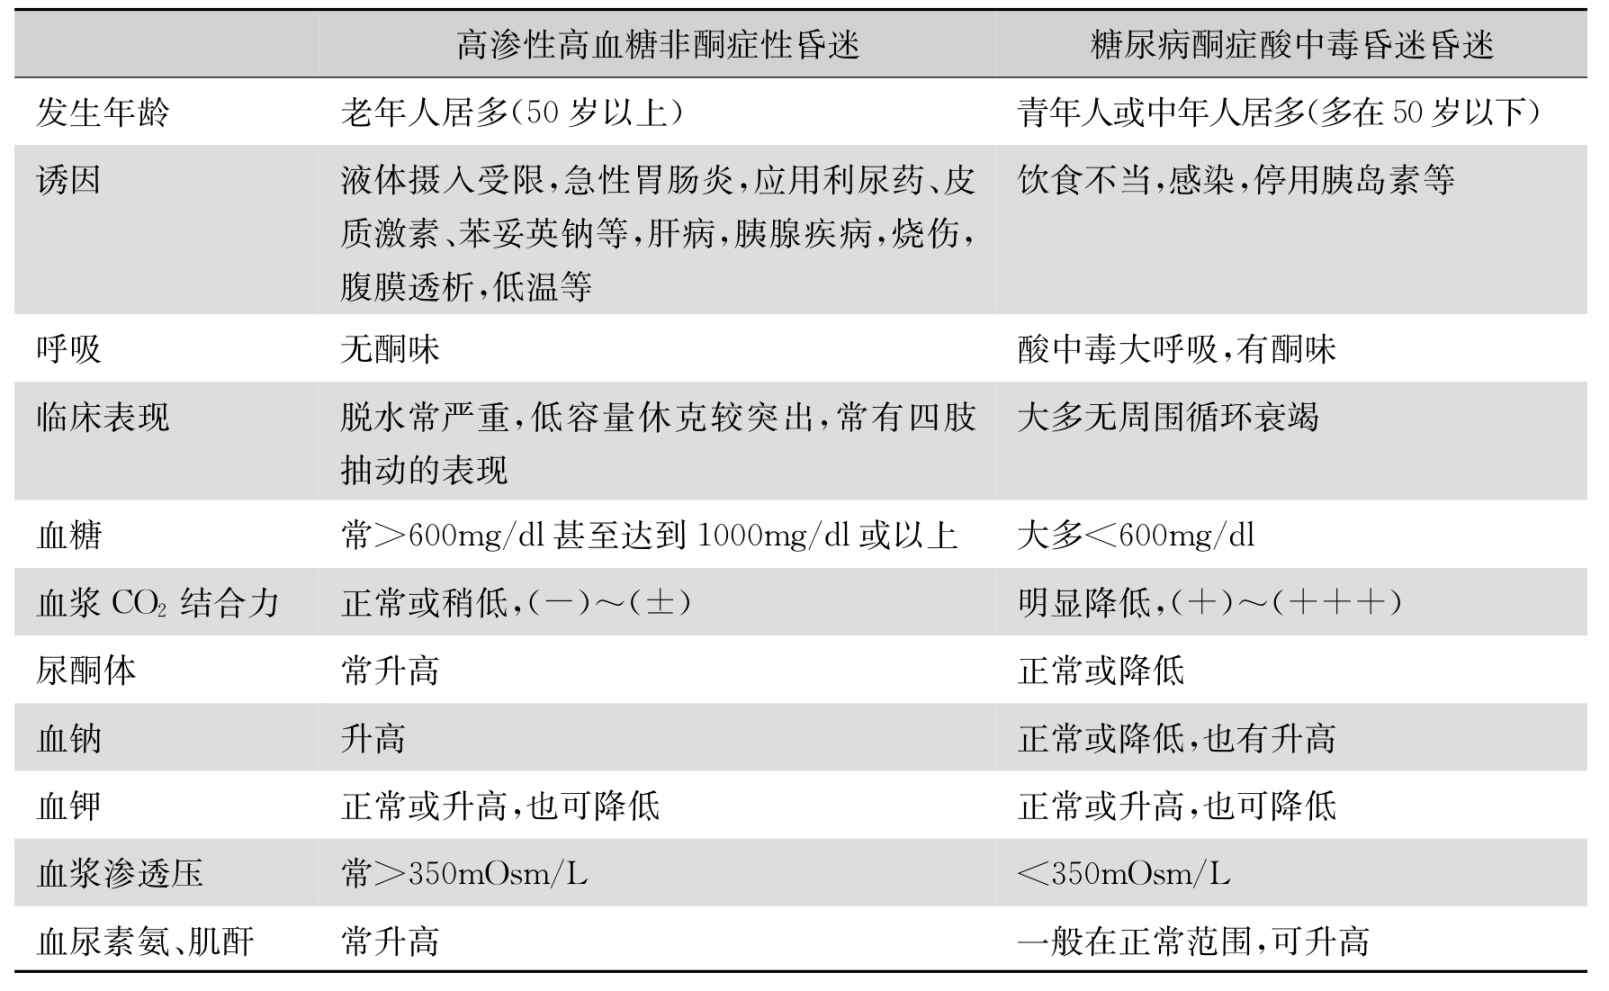
\includegraphics[width=5.94792in,height=3.66667in]{./images/Image00307.jpg}
\end{table}

在外科领域中,高渗性高血糖非酮症性昏迷亦有报告。一组患者8例均无糖尿病史,于脑外伤或脑手术后3~15天发病。作者认为丘脑下部功能障碍导致水、盐、糖等代谢紊乱和内分泌失调是主要的原因,而脱水为其直接原因。临床表现为脱水及神经精神症状,最后导致昏迷。

\subsubsection{七、乳酸酸中毒致意识障碍}

乳酸酸中毒同样多发生于老年患者,可由于尿毒症、糖尿病、细菌性感染、动脉硬化性心脑血管病、肺炎、急性胰腺炎、慢性酒精中毒、休克以及应用氯丙嗪、苯乙双胍等药物而诱发。

大多数糖尿病患者发生乳酸酸中毒是由于服用苯乙双胍。苯乙双胍引起乳酸酸中毒可能是由于抑制氧化磷酸化作用,导致葡萄糖无氧酵解增加所致。这些患者原先已有某种程度的肾功能不全,由于苯乙双胍的排泄取决于肾小球滤过率是否正常,苯乙双胍蓄积达到一定的水平而引起乳酸酸中毒。

病情发展通常相当快,患者可在几小时内发生谵妄而迅速陷入昏迷,伴有酸中毒深大呼吸。缺氧症状也出现,低血压为突出表现之一。患者有上述病史而出现酸中毒与周围循环衰竭表现时,应考虑乳酸酸中毒。

实验室检查血pH值与二氧化碳结合力下降,血乳酸>5mmol/L。血糖水平正常或增高。血酮体与尿酮体正常或轻度增高。由于换气过度所致的呼吸性碱中毒,血中也可有乳酸积聚,故血pH值测定有特殊的鉴别诊断意义。治疗措施主要是静脉滴入碳酸氢钠溶液,必要时尽早行血液透析治疗。

\subsubsection{八、低血糖性昏迷}

低血糖性昏迷可见于应用过量胰岛素的糖尿病患者,或注射胰岛素后未及时进食,也见于使用胰岛素促泌剂或含有胰岛素促泌剂成分中成药的患者。患者在昏迷前常有心慌、出冷汗、眩晕、复视、乏力等感觉,但偶尔在注射胰岛素后突然发生昏迷者也有之。此时需与糖尿病酮症酸中毒昏迷严格区别。主要根据皮肤湿润、瞳孔散大(后期可缩小)、呼吸气息无酮味、尿中无糖与酮体、血糖值在60mg/dl以下、巴宾斯基征阳性等表现。

重症肝病(尤其是原发性肝癌、肝硬化、肝炎)引起低血糖性昏迷也时有之,在乙醚麻醉后尤易激发。

胰岛功能亢进症的低血糖症状发作,如未加以适当的治疗,也易引起低血糖性昏迷。诊断参见第136.1节。

荔枝病是发生于荔枝收获季节的急性疾病。患者常因进食过多荔枝而未进食晚餐,一般在翌晨发病,表现为低血糖症状,注射葡萄糖溶液多有疗效。患者大多为儿童。(参见第138节)

\subsubsection{九、慢性肾上腺皮质功能减退症性昏迷}

慢性肾上腺皮质功能减退症(Addison病)如无并发症,甚少发生昏迷。患者一般只有不同程度的衰弱、乏力、头昏、眼花,有时发生昏厥,主要原因是电解质紊乱、失水、低血压及血糖过低。提示慢性肾上腺皮质功能减退症性昏迷的主要症状是血压急剧下降,在昏迷时甚至可测量不出。

\subsubsection{十、肺性脑病}

肺性脑病常是慢性肺源性心脏病的严重并发症,发病通常在40岁以上,一般见于并发肺部感染或感染恶化之际,应用镇静安眠药为发病的诱因。临床表现为肺、心功能衰竭以及一系列神经精神症状,主要是由于肺功能障碍所致的体内二氧化碳潴留与缺氧。当动脉血二氧化碳分压(PaCO\textsubscript{2}
)增高为正常值的2倍,约达10.6kPa(80mmHg)时,则患者表现为神志模糊、嗜睡(称为二氧化碳麻醉)、肢体颤动、扑翼样震颤、心动过速、视网膜充血等。如PaCO\textsubscript{2}
继续增高为正常值的3倍,即16.0kPa(120mmHg)时,则出现腱反射抑制、病理反射、昏迷、视乳头水肿等。上述症状的出现和PaCO\textsubscript{2}
升高的快慢有关。如PaCO\textsubscript{2}
急骤升高,则症状出现较快;如PaCO\textsubscript{2}
缓慢升高,则症状出现较慢。

肺性脑病的诊断,可根据肺心病伴有失代偿性呼吸性酸中毒的存在,上述临床表现,血分析检查PaCO\textsubscript{2}
增高与动脉血氧分压(PaO\textsubscript{2}
)降低,并除外其他原因的中枢神经系统疾病而确定之。

\protect\hypertarget{text00372.html}{}{}

\subsection{163.3 水、电解质平衡紊乱}

\subsubsection{一、稀释性低钠血症}

此症起病较缓,但也可急性起病。主要临床表现为厌食、表情淡漠、恶心、呕吐、嗜睡、尿量减少、水肿、体重增加、周围静脉充盈饱满、低血压。血中非蛋白氮可升高,血清钠降低(130mmol/L以下),尿钠浓度低。血清钠下降至120mmol/L左右时,患者常有易激动与神志错乱。若降至110mmol/L或以下时,患者常有嗜睡或昏迷,且出现全身性抽搐。如不立即采取适当措施,则患者可致死亡。

此症主要见于重度及病程较长的慢性充血性心力衰竭或肝硬化顽固性腹水患者,伴有肾滤过率降低,同时严格限制食盐并输入过多水分的情况。细胞外液的水分相对增多,水肿显著,少尿而患者并无口渴的感觉,这种情况也称水中毒。

水中毒尚可见于慢性肾上腺皮质功能减退症的患者,或垂体功能减退症患者接受药物治疗而又大量饮水时,以及急性肾衰竭患者少尿期未限制水入量等情况,此时肾血流量不足,未能正常地排出水分。

\subsubsection{二、低氯血性碱中毒}

此症在内科方面主要见于充血性心力衰竭时不适当地应用汞利尿剂,致血中氯化物过度丧失所致。此外,也可见于幽门梗阻兼有剧烈呕吐等情况。患者表情淡漠、厌食、乏力、意识蒙眬或错乱,更严重时发生搐搦(由于血中钙离子减少)及昏迷。血生化检查血清氯明显降低(常在90mmol/L以下),血清钠往往正常(幽门梗阻时可减少),二氯化碳结合力升高。尿pH值趋向碱性,则表明逐渐趋向碱中毒。每日多次用pH试纸测定尿pH值,可及早发现碱中毒。如充血性心力衰竭患者应用利尿剂渐而失效,水潴留及心力衰竭现象反而加重,而患者无感染、心肌梗死、肺栓塞、肾功能不全等并发症时,应考虑此症的可能性。

\subsubsection{三、高氯血性酸中毒}

高氯血性酸中毒可见于充血性心力衰竭时、过量应用氯化铵所引起。氯化铵在肠道被吸收之后,铵在肝内与二氧化碳结合成为尿素,产生大量氢离子,致使血液酸化,血中碳酸氢盐含量下降。氯离子从肾脏排出时又携走钠离子,血中二氧化碳结合力不断下降,结果导致高氯血性酸中毒,血清氯含量常超过110mmol/L。钾离子也可大量从尿液排出而致血清钾降低。

高氯血性酸中毒的早期临床表现是厌食、恶心、呕吐、乏力等症状,进一步则可出现神志不清、呼吸深大,如不及时救治则可昏迷。

高氯血性酸中毒尚可见于慢性肾盂肾炎、肾小球性酸中毒、Fanconi综合征、输尿管结肠吻合术后等情况。慢性肾盂肾炎时肾小球滤过功能仅有轻度损害,而肾小管排酸功能显著减退,致血中碳酸氢盐不断降低,氯离子重吸收增加,则可产生高氯血性酸中毒。输尿管结肠吻合术后尿液在结肠中潴留,氢、氯和铵离子等被吸收,再经肾脏排泄,形成肠道肾脏循环,肾脏排酸负担加重,肾小管排酸功能减退及氯离子等的渗透性利尿,使碱基不断耗损,结果可发生高氯血性酸中毒。

\protect\hypertarget{text00373.html}{}{}

\subsection{163.4 外因性中毒}

对有明确毒物接触史的昏迷患者诊断为外因性中毒并不困难,而无(或不注意)毒物接触史则易误诊。如患者素来健康,突然发生头痛、头晕、恶心、呕吐、腹痛、抽搐乃至昏迷等症状,需注意急性中毒的可能性。又如慢性疾病突然发生昏迷而不能用原有疾病解释其原因时,也应考虑急性中毒的可能性。如有毒物接触史或身边遗有剩余毒物,则可能性甚大。当患者昏迷时,向其家属、同事或其他有关方面了解,往往也能提供诊断的线索。应立即取患者的剩余可疑毒物、排泄物(呕吐物、尿、粪)甚至血液作毒物分析,以期迅速确定诊断。表\ref{tab49-3}可作为外因性急性中毒诊断与鉴别的参考。

\subsubsection{163.4.1 工业毒物中毒}

\paragraph{一、一氧化碳中毒}

一氧化碳中毒俗称煤气中毒,患者中毒场所的调查有助于诊断。此病通常发生于冬季,中毒场所必有煤炉或漏气的煤气管。患者颜面粉红、口唇樱红、呼吸与脉搏加快,严重者发生惊厥、昏迷、瞳孔散大,呈潮式呼吸,可因心脏与呼吸受抑制而死亡。静脉血呈鲜红色泽,分光镜检可证明有碳氧血红蛋白。简单的化验方法为采取患者的血液数滴,加入蒸馏水,再加入10\%氢氧化钠溶液数滴,如有碳氧血红蛋白存在,则所呈的淡红色不变,如为正常血液,则变为带黄绿的棕色。

\begin{longtable}{c}
 \caption{外因性中毒昏迷某些表现的鉴别诊断意义}
 \label{tab49-3}
 \endfirsthead
 \caption[]{外因性中毒昏迷某些表现的鉴别诊断意义}
 \endhead
 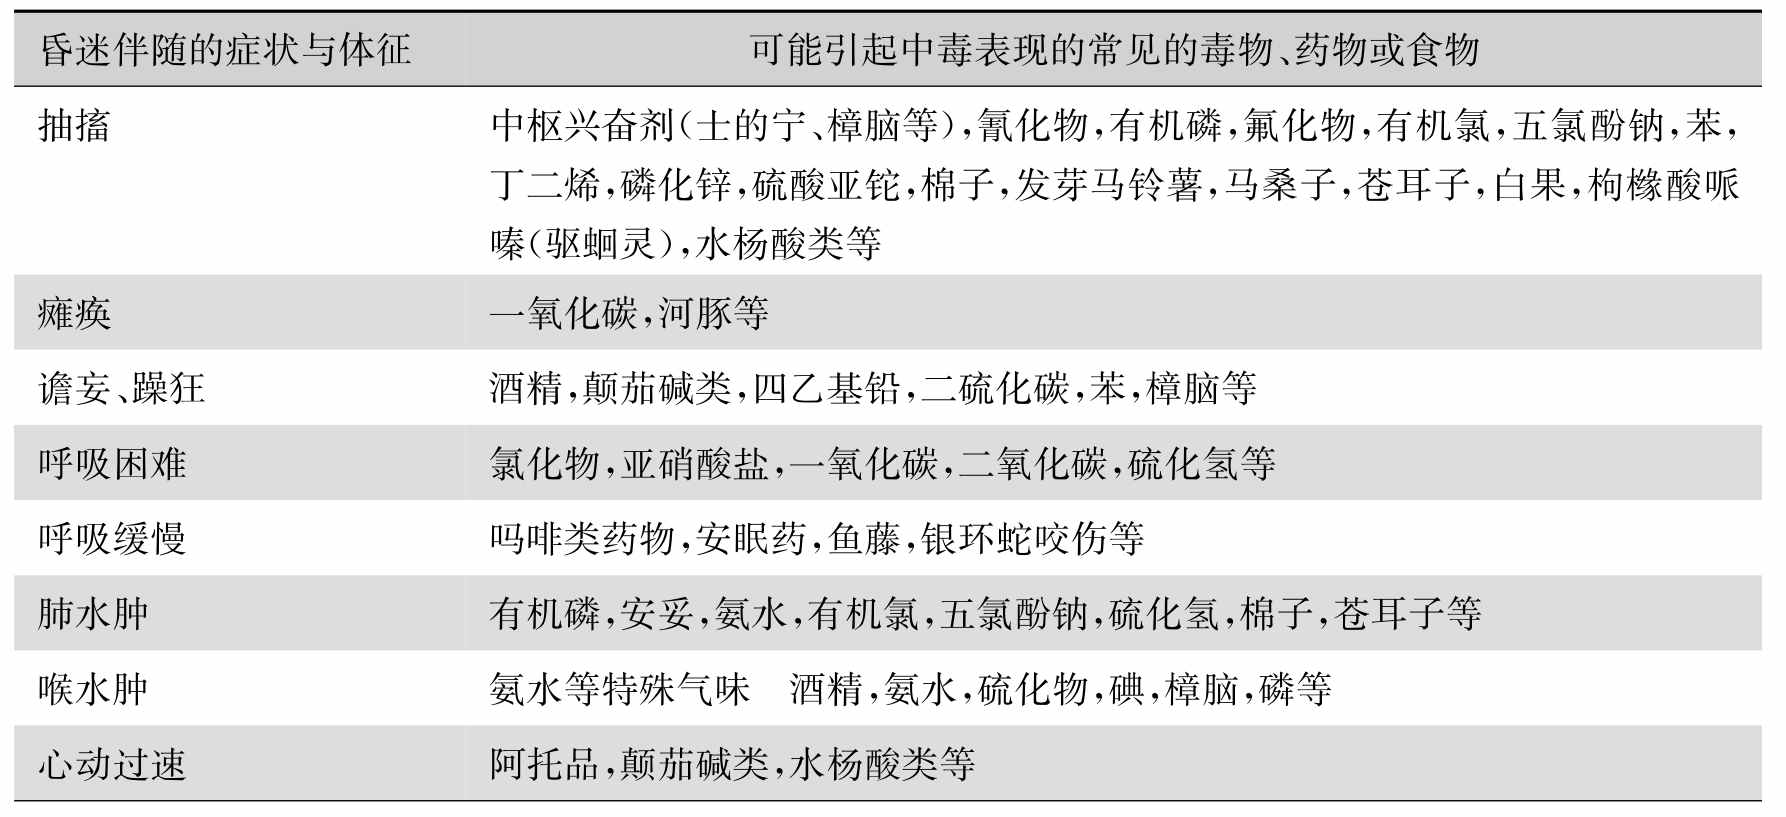
\includegraphics[width=\textwidth,height=\textheight,keepaspectratio]{./images/Image00308.jpg}\\
 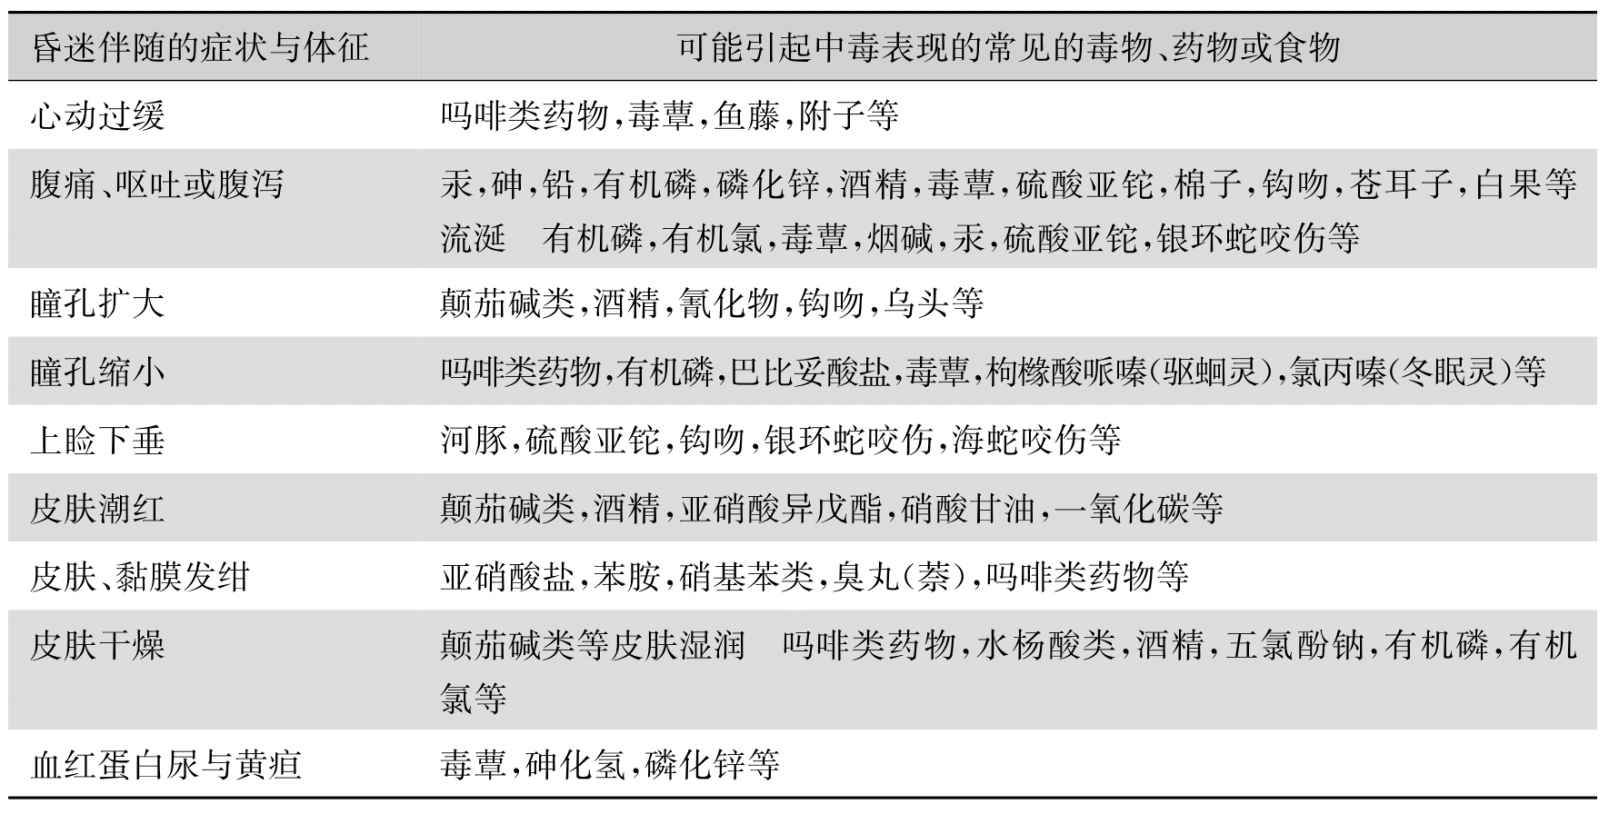
\includegraphics[width=\textwidth,height=\textheight,keepaspectratio]{./images/Image00309.jpg}
 \end{longtable}

一氧化碳急性中毒后不少病例发生神经精神症状,主要表现是帕金森综合征、舞蹈症、痴呆、木僵、精神错乱、躁动不安、抽搐、肢体瘫痪、失语等。大部分病例是昏迷清醒后数天至两个月内发生,有时可误诊为其他原因所致的神经精神病;小部分病例上述症状是昏迷后延续出现而无间歇期。

\paragraph{二、急性硫化氢中毒}

由于跌入化粪池、腌菜池引起的急性硫化氢中毒,临床上均有报告,但也可由于工业事故所致。硫化氢由呼吸道吸收后作用于神经系统,极大量则引起意识模糊、谵妄、抽搐与昏迷。最后可因呼吸麻痹而死亡。病程迁延者可以发生中毒性肺炎与肺水肿。

\paragraph{三、急性苯中毒}

苯是工业上广泛使用的一种溶剂和原料,特别是油漆、喷漆中含量甚高。有人报道吸入高浓度的苯蒸气,可引起急性中毒死亡,发生在通风不良处从事油漆或喷漆操作过程中。轻症急性中毒时患者呈醉酒状,出现兴奋、颜面潮红、头晕、头痛、恶心、呕吐、行走蹒跚、手足感觉异常及胸部紧迫感等症状,并可因苯的局部刺激而引起结膜炎。严重中毒时出现神志不清、昏睡、脉搏细弱、血压下降、瞳孔散大、对光反射消失,甚至昏迷、抽搐、全身皮肤出血,最后可因呼吸中枢麻痹而死亡。突然大量吸入时,可在数分钟内因昏迷与呼吸麻痹而死亡。

\paragraph{四、急性苯胺中毒}

急性苯胺中毒曾见于喷漆、印染及化工工人。苯胺中毒主要由于皮肤与黏膜的直接接触而吸收,后者常由于呼吸道吸入所引起。主要症状为眩晕、头痛、嗜睡、呼吸困难、恶心、呕吐、体温与血压下降、发绀,严重者有神志模糊、抽搐甚至死亡。

\paragraph{五、急性丁二烯中毒}

丁二烯是人造橡胶的原料,是带有甜味的气体,短期内大量吸入对黏膜有强烈刺激作用,表现为眼痛、喉痛、刺激性咳嗽、流泪、畏光、胸闷与呼吸困难。吸收后损害中枢神经系统,引起头痛、头晕、乏力。重症者出现烦躁不安、震颤、昏迷与抽搐。

\paragraph{六、急性二硫化碳中毒}

由于工业事故而在短期内吸入大量二硫化碳蒸气时,可引起急性中毒性脑病,表现为谵妄、昏迷、抽搐,甚至呼吸麻痹。

\subsubsection{163.4.2 农药类中毒}

\paragraph{一、急性有机磷中毒}

有机磷可从消化道、呼吸道、皮肤进入人体而引起中毒,以对硫磷(1605)、内吸磷(1059)、敌百虫、敌敌畏等中毒多见。有机磷能抑制胆碱酯酶的活性,致乙酰胆碱在体内蓄积过多而引起中毒症状,主要表现为胃肠道与神经系统方面的损害。

重度有机磷农药急性中毒患者呈昏迷状态,需注意与中暑、乙型脑炎、中毒型菌痢等相鉴别。有时患者被送入院时多汗期已过,临床表现为昏迷与瞳孔缩小,需注意与吗啡类药物或巴比妥类药物中毒相鉴别。细致采取病史和作血胆碱酯酶活性测定(重度有机磷农药急性中毒时一般降至正常值的30\%以下),有助于诊断。

\paragraph{二、急性有机氯中毒}

有机氯可从消化道、呼吸道进入人体而引起中毒,以由于六六六、二二三(氯苯乙烷)等引起者为多见。急性中毒主要侵犯神经系统,也可引起肝、肾损害。

1.轻度中毒乏力、头痛、头晕、厌食、视力模糊、恶心、呕吐、腹痛等。

2.中度中毒多汗、流涎、呕吐、肌肉震颤、抽搐、发绀等。

3.重度中毒出现癫痫样发作、昏迷,大量吸入时可发生肺水肿。可因呼吸衰竭或心室颤动而死亡。

\paragraph{三、急性有机汞中毒}

有机汞中毒可由于误服或吸入有机汞农药(赛力散、西力生、新西力生等)所致。急性中毒主要表现为胃肠道、神经系统与感觉器官方面的症状。患者自觉口有金属味、流涎、恶心、呕吐。神经系统症状表现为中毒性脑病,出现头痛、头晕、肌肉震颤、共济失调、言语困难,甚至四肢瘫痪。感觉器官症状则有视力模糊、视野缩小、听力减退、嗅觉障碍等。心动过速或过缓,可出现房室传导阻滞。严重者可发生昏迷、抽搐而死亡。

\paragraph{四、急性氯化苦中毒}

氯化苦(三氯硝基甲烷)为农药熏蒸剂,有严重的刺激性,短期内吸入高浓度时可引起急性中毒。初期表现为头昏、头痛、恶心、流泪、流涕、咽干、气促等症状,继而出现呼吸困难、胸闷、胸痛、发绀,严重者出现昏迷。肺部听诊有干啰音。恢复后常有肝大与触痛。

\paragraph{五、急性磷化锌中毒}

磷化锌是一种剧毒的杀鼠剂,误食之可引起急性中毒。磷化锌遇酸即分解成有剧毒的磷化氢,对胃肠黏膜有腐蚀作用,引起腹部不适、厌食、恶心、呕吐、血便。吸收以后引起中枢神经系统损害,使患者出现头晕、烦躁、四肢抽搐、发绀、昏迷等症状。毒物经肝脏解毒、肾脏排泄,引起肝、肾损害,出现黄疸与血尿。

\paragraph{六、急性硫酸亚铊中毒}

硫酸亚铊是白色结晶体,能溶于水,有剧毒。致死量在0.2~1.0g之间,一般用作毒鼠药及脱毛剂。误服可引起死亡。重症急性中毒表现为急性胃肠炎症状,如恶心、呕吐、腹绞痛、下痢等,其他有溃疡性口炎、流涎、口有金属味。吸收后损害神经系统与心肌,可引起四肢麻木、斜视、眼睑下垂、瞳孔散大、血压上升、心肌损害、窦性心动过速、发绀、震颤、四肢抽搐与昏迷。

\subsubsection{163.4.3 药物类中毒}

\paragraph{一、巴比妥酸盐中毒}

巴比妥酸盐中毒时,患者平静进入昏迷。患者全身肌肉松弛,呼吸浅慢,体温降低,脉搏微弱,瞳孔缩小,重症者反射消失。巴宾斯基征有时阳性。在昏迷期的患者,亦可无并发肺炎而高热达41℃。诊断需根据服毒史以及胃内容物或尿液化学定性分析。

\paragraph{二、吩噻嗪类中毒}

氯丙嗪、乙酰丙嗪、奋乃静等轻度中毒,表现为嗜睡、软弱、血压轻度下降、体位性低血压。剂量较大时,有恶心、口干、肌肉震颤与抽搐、瞳孔缩小、心动过速、体温下降;严重中毒时有深昏迷、休克。长期服用氯丙嗪可使耐受量增加,例如精神病患者,曾有一例顿服氯丙嗪5000mg,经及时救治而痊愈。诊断未明的病例可作尿氯丙嗪定性试验以证实之。

\paragraph{三、急性吗啡类药物中毒}

急性吗啡类药物中毒的临床特征为瞳孔缩小如针眼,脉搏与呼吸减慢,常有发绀,有时出现巴宾斯基征,昏睡或昏迷。严重者出现潮式呼吸,可因呼吸抑制而死亡。诊断需根据用药史、临床症状及胃内容物与尿液化学分析。

\paragraph{四、颠茄类中毒}

颠茄类包括颠茄、莨菪碱、曼陀罗素、阿托品等。中毒的主要表现是颜面潮红、口干、皮肤干燥、发热、视力模糊、瞳孔散大、心搏过速等。重症者发生谵妄与昏迷。

颠茄在秋季结美丽的橙红色果实于旷野间,儿童误服而致中毒者也曾见之。

\paragraph{五、急性醇中毒}

急性醇中毒甚少引起深度昏迷。患者发病前有酗酒史,患者的呼吸气息、呕吐物、血液与尿均有醇味,可作诊断之助,需注意者是以饮酒为诱因的脑出血,但后者有神经学病征(偏瘫、巴宾斯基征)可为鉴别之助。

\subsubsection{163.4.4 植物类中毒}

\paragraph{一、氯化物中毒(包括木薯、苦杏仁中毒)}

氰化物、木薯和含氰苷类种子(苦杏仁、枇杷仁、桃仁、樱桃仁)所致的中毒,并非过于少见。其发病机制是因氰酸离子被吸收后即与细胞色素氧化酶的铁结合,从而破坏细胞色素氧化酶的作用,抑制组织呼吸,使机体陷于窒息状态所致。苦杏仁中毒的潜伏期多为1~2小时,木薯中毒为2~9小时不等。一般急性中毒可分为四期:

\subparagraph{1.前驱期}

患者有咽部热辣感与麻木感、流涎、恶心、呕吐、头痛、头晕、耳鸣、乏力、心悸、胸闷、肌肉震颤等症状。

\subparagraph{2.呼吸困难期}

出现胸闷、心悸、气促、血压升高、脉搏缓慢、瞳孔散大、神志模糊乃至昏迷。

\subparagraph{3.痉挛期}

全身性阵发性抽搐、大小便失禁、意识丧失、体温下降、出汗。

\subparagraph{4.麻痹期}

深度昏迷、呼吸浅慢乃至停止。临终前均无明显发绀。

\paragraph{二、急性棉子中毒}

棉子所含的毒物为棉子油酚,大量进食时可引起急性中毒。潜伏期大多数为2~4天,短者仅数小时,而长者在6~7天后始发病。中毒较轻者出现恶心、呕吐、厌食、便秘、腹胀或腹痛等胃肠症状,以及乏力、头昏、精神不振等全身症状。严重者可发生嗜睡或烦躁不安、抽搐、昏迷等中枢神经系统症状,以及胃肠道出血。部分患者可发生肺水肿、肝性脑病与心、肾功能不全,最后可死于呼吸与循环中枢衰竭。

\paragraph{三、钩吻中毒}

钩吻也称断肠草、水莽草、大茶药、雷公藤,有剧毒,民间有作治风湿药,可引起中毒。主要的毒性症状是口、咽与腹部烧灼痛、厌食、呕吐、腹泻、少尿或无尿、蛋白尿,以及吞咽困难、眩晕、复视、视力减退、眼睑下垂、瞳孔散大、肌肉软弱、四肢麻木、言语含糊等神经系统症状。严重者可发生昏迷,并可因肾衰竭与休克而死亡。

\paragraph{四、苍耳子中毒}

苍耳子及其幼芽均含有毒性颇强的毒物。轻度中毒表现为乏力、精神萎靡、头昏、头痛、厌食、恶心、呕吐、便秘或腹泻等。较重病例则除上述症状之外,尚有嗜睡或烦躁不安、心率增快或减慢、微热、出汗,或有轻度黄疸、肝大与触痛等。更严重者则发生昏迷、抽搐、休克、尿闭、胃肠道大出血或出现肺水肿、肝性脑病等,以致死亡。血清谷-丙转氨酶均有不同程度的增高。尿中可出现蛋白、细胞与管型。

\paragraph{五、白果中毒(参见第74.1节)}

\subsubsection{163.4.5 动物类中毒}

毒蛇咬伤参见第120节。

\protect\hypertarget{text00374.html}{}{}

\subsection{163.5 物理性及缺氧性损害}

\subsubsection{一、热射病(中暑性高热)}

人体在高温和热辐射的长时间作用下,尤其是当空气温度高、风速小时,体温调节发生障碍而发生热射病。在强体力劳动、久病后体弱、产后、老年人、不惯在炎热的环境下工作、饮水不足以及穿衣过多等情况下较易发生。初起表现为疲乏、头痛、头晕、口渴、多汗、脉搏与呼吸加快等症状。患者迅速昏倒,脉搏微弱,呼吸浅表,血压下降,面容苍白,皮肤潮冷,口腔温度低于正常而肛温微升,此类表现称为循环衰竭型中暑。另一类表现是患者在短期内意识不清、烦躁不安、抽搐,继而昏睡、昏迷,颜面潮红,皮肤干燥灼热,瞳孔缩小、反应迟钝,脉快,呼吸浅速,体温可高达41℃以上,称为高热昏迷型中暑。晚期瞳孔散大,对光反射消失。实验室检查可发现血浆二氧化碳结合力降低,氯化物减少。

老年人发生热射病时,首先需与脑出血相区别。脑出血时常先出现昏迷,然后有发热,同时出现肢体的弛缓性瘫痪。

乙型脑炎也流行于炎热季节,并出现高热与昏迷,与热射病的鉴别是乙型脑炎有神经系统损害征象,脑脊液的蛋白质与细胞数均增加。热射病与脑型疟疾的鉴别则主要依据后者有流行病学史,昏迷发生较慢,周围血中可检出疟原虫。

\subsubsection{二、日射病}

日射病不同于热射病,是由于日光或强烈的辐射热相当长时间地作用于人体引起,主要发生于烈日下不戴帽从事体力劳动、行军及其他作业的人,在有大量热辐射的高温车间工作的人有时也可发生。日射病并非体温调节障碍的结果。日光的辐射热在穿过头皮和颅骨时,99\%被其阻留,能达到脑膜者约1\%。此量虽小,也足以引起脑膜和大脑充血及其他损害。

发病急骤,开始时有乏力、剧烈头痛、头晕、耳鸣等症状,呕吐也较多见。继而血压下降,脉搏与呼吸加快,出汗,重症者发生惊厥,最后陷入昏迷。患者体温正常或轻度升高。

\subsubsection{三、触 电}

重症的触电可立即发生昏迷,呼吸中枢麻痹而致呼吸停止,但心搏仍存在。皮肤发绀而厥冷,血压下降甚剧。如合并心室颤动,则心音也消失。

\subsubsection{四、高山性昏迷}

人从平原地带如未经适应锻炼而进入高山或高原地区,在短期内可因机体急性缺氧而发生昏迷。迅速缺氧时首先影响中枢神经系统,开始是兴奋,渐入抑制,表情淡漠、反射迟钝、不思饮食、嗜睡,最后发生昏迷------高山性昏迷。脑脊液检查可有压力增高,蛋白质、糖、细胞数一般无改变。心肺及血象检查通常无显著异常。约半数患者血压升高。由于呼吸频数、肺泡二氧化碳张力降低,可引起呼吸性碱中毒。缺氧也可增加肺毛细血管的通透性,从而导致急性肺水肿。

\protect\hypertarget{text00375.html}{}{}

\section{164 颅内病变}

\subsection{164.1 脑感染性疾病}

参见第163.1节。

\protect\hypertarget{text00376.html}{}{}

\subsection{164.2 脑血管疾病}

\subsubsection{一、脑出血}

脑出血是指原发性非外伤性脑实质内出血,也称自发性脑出血,占全部脑卒中的20\%~30\%,小脑出血及脑桥出血广义上也属于脑出血,分别在本节述及。

脑出血多发生在50岁以上、血压控制不良的高血压患者。部分患者有家族性高血压病史或脑血管意外病史。最常见的病因是高血压性脑内小动脉硬化,国外某组225例脑出血的尸检结果证实,60\%是由于高血压性动脉硬化所引起,其他较少见的原因是颅内动脉瘤、脑血管畸形、血液病、子痫、脑肿瘤破裂出血等。

国内报道一组脑出血中,发病时有高血压者占94.9\%,意识障碍占79.5\%,较梗死性血管病多见且严重,在鉴别诊断时值得注意。意识障碍越深,死亡率越高。

本病起病多数较突然,通常在用力、兴奋、情绪激动等状态下发病,症状在数分钟至数小时内达高峰。临床主要表现为两大类症状,即全脑症状(颅内压力增高所致)以及神经系统定位症状(出血对某部分脑组织的刺激和破坏所致)。

全脑症状中最突出的症状是不同程度的昏迷,这也是与其他类型急性脑血管疾病鉴别的要点。根据几组病例的统计,有昏迷者约占70\%~88\%。大部分患者开始即有昏迷,少数病例其昏迷逐渐发生。昏迷的程度与出血量的多寡以及出血的部位有很大关系;有人认为,如病灶接近第三脑室的中央灰、白质或丘脑核,则昏迷最易发生。如出血流入脑室,则常呈深度昏迷。如血肿波及或压迫丘脑下部时可刺激丘脑下部的自主神经中枢,使其功能紊乱,导致上消化道黏膜的血管急性扩张出血,称应激性溃疡出血。

神经系统的局部症状根据出血部位而定。出血可发生在大脑皮质、皮质下、基底节区、脑干、小脑、脑室等部位。基底节区是最常见的好发部位,约占60\%~70\%,其中壳核出血约占60\%,丘脑出血约占10\%,带状核和尾状核出血少见。

\paragraph{(一)壳核出血}

即内囊外侧型出血,多由外侧豆纹动脉破裂引起,血肿常向内扩展压迫内囊,出血量大可致昏迷。由于行经内囊的皮质脊髓束、皮质脑干束、脊髓丘脑束和视放射受累,患者出现病灶对侧偏瘫以及对侧下部面肌瘫痪(面神经核上性瘫痪)。至于对侧舌肌的核上性瘫痪和对侧偏身感觉障碍在患者昏迷时不易查出,病灶在优势半球者可有运动性失语。急性期偏瘫多为弛缓性。患者两眼球常向病灶侧凝斜。不少患者的另一侧肢体也有锥体束征,乃因脑水肿所致。

\paragraph{(二)丘脑出血}

即内囊内侧型出血,是丘脑穿通动脉或丘脑膝状动脉破裂所引起,典型的症状是偏身感觉异常,血肿向外压迫或损伤内囊可引起病灶对侧偏瘫、偏身感觉障碍和同向偏盲,部分患者可伴有偏身自发性疼痛或感觉过度;优势半球出血可有运动性失语,非优势半球出血可有体像障碍及偏侧忽视症。部分患者还可出现精神障碍,表现为情绪低落、情感淡漠或视幻觉、类精神分裂样症状及记忆和认知功能减退。血肿向内破入脑室称继发性脑室出血,可引起昏迷、高热和瞳孔改变。血肿向下扩展压迫丘脑下部和脑干,亦可出现昏迷、高热和上消化道出血,最后继发脑干功能衰竭而死亡。

\paragraph{(三)脑叶出血}

即皮层下白质出血,老年患者常由高血压动脉硬化或淀粉样变血管病所引起,青壮年多为先天性脑动静脉畸形或先天性动脉瘤破裂所致。出血量大时常有不同程度的昏迷,且伴有相应脑叶功能受损的表现,如额叶出血可出现精神异常、摸索、强握等;颞叶出血可出现幻视、幻听、感觉性失语等;顶叶出血则为肢体感觉障碍、失用、失认、体像障碍等;枕叶出血可出现皮质盲。

\paragraph{(四)脑干出血}

占全部脑出血的10\%左右,主要由旁正中动脉和短旋动脉破裂所致。按出血部位可分为中脑出血、脑桥出血和延髓出血。其中以脑桥出血最常见,占脑干出血的80\%以上,病变部位多位于脑桥中部的基底部和被盖部之间。临床表现与出血量有关,当出血量达3ml以上时,患者很快陷入昏迷(脑桥内网状结构受损)、高热(脑桥内两侧交感神经纤维受累)、四肢瘫痪、针尖样瞳孔(脑干与视丘下部调节体温的纤维破坏)、呼吸节律不整甚至呼吸停止,并可伴多脏器功能衰竭;多数患者于短期内死亡,临床不易确诊。如出血量在1.5ml以下,患者可不昏迷。部分患者出现抽搐,少数病例在起病时有构音障碍、吞咽困难。此时细致检查或可发现一侧面肌麻痹和对侧肢体弛缓性瘫痪的交叉性特点,患者的头部和两眼斜向偏瘫侧。并非所有的患者皆表现为交叉性瘫痪的典型征象,因出血和水肿可很快扩展至脑桥另一侧,或开始起病即为双侧。瞳孔多数缩小如针尖,眼球可上、下浮动或固定于中间位置。脑脊液多为血性。临床遇有突然昏迷、呕吐、四肢弛缓性瘫痪的中、老年患者,应疑及脑桥出血。若患者双侧瞳孔极度缩小以及中枢性高热,则进一步支持本病的诊断。后期患者双侧瞳孔散大,对光反射消失,四肢强直。由于出血及水肿波及延髓生命中枢,呼吸明显障碍,循环衰竭,病情危笃。经抢救度过昏迷期者,可表现为四肢瘫、双侧性面神经和展神经麻痹、不能言语、不能进食、不能做各种动作、不能自解大小便,仅可做眼球上、下运动,貌似闭锁综合征。中脑出血和延髓出血均比较少见。中脑少量出血时表现为昏睡、单侧或双侧动眼神经麻痹、眼位异常、单侧或双侧锥体束征。大量出血者表现为深昏迷,双侧瞳孔散大,四肢瘫痪,可在短期内死亡。延髓出血常由脑桥出血扩展而来,表现为突然昏迷,血压下降,呼吸节律不整或呼吸停止,心律失常,亦可迅速死亡。

\paragraph{(五)小脑出血}

并非罕见,其发生率约占脑出血的10\%左右,病因最常为高血压及动脉硬化,故患者大多为60岁以上的老年人;较少见的病因是先天性血管畸形,其发病年龄常在15~40岁。有人认为血管畸形愈小,愈易出血,有时剖检找不到原因,可能出血原发于微细的血管畸形,后者为出血灶所掩盖。小脑出血的症状无一定的规律,取决于出血部位、出血量的多寡以及病变对邻近组织的压迫。临床表现可分三型:

\subparagraph{1.暴发型(闪电型)}

约占20\%。常为蚓部出血破入第四脑室。患者突然昏迷,呕吐,四肢弛缓性瘫,脉细,呼吸弱,瞳孔散大,光反射消失,可在数小时内死亡。伴急性肺水肿者可在数分钟内死亡。

\subparagraph{2.恶化型}

占多数。出血后逐渐流入脑室,或破入蛛网膜下腔阻塞脑脊液通道。大部分病例起病突然,初起可有头晕或眩晕、头痛、呕吐、共济失调等,逐渐出现脑干受压症状,如眼球协同运动障碍、面瘫、呼吸障碍等。其后患者出现不同程度的意识障碍,后期可有去脑强直。可在数日或一二周内逐渐加重而死亡。

\subparagraph{3.良性型}

占少数。多为小脑半球的中心部少量出血,缓慢进展,临床表现似小脑肿瘤。常表现为头痛、头晕、呕吐、眼球震颤、共济失调,角膜反射常早期消失。如出血停止可渐被吸收,逐渐恢复,或遗留某些后遗症。如出血继续发展,则转为恶化型。

小脑出血最常见的病征是眼症状,可见眼球浮动、眼球分离性偏斜或上、下偏斜;注视麻痹;眼球震颤;瞳孔不等大或忽大忽小,对光反射减弱;角膜反射较早消失。患者常有三项体征同时存在,名为三联症。最常见的三联症是:①瞳孔缩小或一侧扩大;②注视麻痹;③呼吸障碍。其他三联症是:瞳孔缩小或不对称、注视麻痹、轻偏瘫,或注视麻痹、周围性面瘫、共济失调。由于小脑出血常继发脑干受压,故呼吸障碍也为常见的病征。小脑出血易溃入第四脑室,继发脑室出血及蛛网膜下腔出血,脑脊液压力增高,据统计血性脑脊液为47\%~90\%。小脑出血后因患者大多迅速昏迷,因而小脑损害的病征如步态不稳、共济失调、构音障碍等有时存在,有时不易查出,临床上难以完全依靠小脑病征的有无来确诊。

在CT、MRI问世之前,小脑出血的诊断相当困难,经常误诊为脑出血和蛛网膜下腔出血。小脑出血的主要诊断根据为:①患有高血压及动脉硬化的老年人,少数患者为青壮年;②发病突然,大多数患者在初起时头痛特别是枕后痛、眩晕、呕吐,其后迅速出现不同程度的意识障碍;③瞳孔缩小或不对称,注视麻痹,眼球浮动或分离,角膜反射早期消失;④呼吸障碍尤以呼吸暂停为多见;⑤血性脑脊液及脑膜刺激征;⑥如有小脑病征则进一步支持本病的诊断;⑦头颅CT检查可发现小脑内高密度影,能明确出血部位、范围和第四脑室受压情况,对指导治疗、估计预后有重要价值。临床一旦怀疑小脑出血,应尽快行头颅CT检查。头颅MRI检查可明确出血部位、范围和第四脑室受压情况;T1加权像呈等信号,T2加权像呈略高信号,但检查耗时长,不属首选。小脑出血主要需与脑出血、原发性蛛网膜下腔出血、脑桥出血等相鉴别。典型的大脑半球出血常有偏瘫和面神经的核上性瘫;患者眼球多向病灶侧偏斜;原发性蛛网膜下腔出血患者多为青壮年,意识障碍不深,且较易恢复,眼球浮动或分离性偏斜少见。脑桥出血常有四肢及脑神经瘫痪,瞳孔缩小如针眼,中枢性高热等,可与小脑出血鉴别。小脑出血与小脑梗死的鉴别是:后者的脑干受压症状较慢,脑脊液非血性,压力不高,脑超声波检查侧脑室不扩大。

\paragraph{(六)继发性脑室出血}

蛛网膜下腔出血,血肿破入脑室引起脑室出血称继发性脑室出血。症状因出血部位、脑室积血量及是否阻塞脑脊液通路而异,如出血量大,病情危笃,呈深昏迷、高热、双侧瞳孔缩小如针眼,与脑桥出血相仿,不同者是继发性脑室出血很早就出现四肢阵发性强直性抽搐,死亡的发生更快。直接由脉络丛血管出血或室管膜下1.5cm处出血破入脑室者为原发性脑室出血,较少见,出血量少时表现为头痛、呕吐、颈项强硬,Kernig征阳性,意识清楚,预后良好。如出血量大,则表现与继发性脑室出血或脑桥出血雷同,但脑的局灶症状缺如。脑出血经由脑室或穿破脑实质流入蛛网膜下腔,称继发性蛛网膜下腔出血,刺激脑膜,约半数患者出现颈强硬及Kernig征阳性。少数患者发生全面性癫痫或部分性癫痫发作。病情较单纯性脑实质出血严重,且预后更差。

不少患者伴有心肌损害、肺炎、电解质平衡障碍、蛋白尿和糖尿、周围血白细胞增多等。患者的体温逐渐升高,极期可达40℃以上。

辅助检查:①头颅CT,临床一旦怀疑脑出血,应尽快检查,可发现脑内相应部位的高密度影,能明确出血部位、范围和脑水肿的程度及脑室系统情况,对指导治疗、估计预后有重要价值,对判断昏迷发生的原因也有意义;②头颅MRI检查,可明确出血部位、范围和脑水肿及脑室情况;T1加权像呈等信号,T2加权像呈略高信号,但检查耗时长,不同时段有不同的改变,且图像不如CT易于判断,不属首选;③脑血管造影(DSA、CTA、MRA)可显示血管走行的移位,有的尚可发现脑动脉瘤或血管瘤,但急性期较少使用;④腰穿脑脊液压力增高,多呈均匀血性,但血肿没破入脑室或蛛网膜下腔时,脑脊液可为非血性,随着CT的临床应用,本项检查已不属常规检查项目。

综上所述,脑出血的主要诊断根据为:①患者大多数是患有高血压及动脉硬化的中、老年人;②常在用力或兴奋情况下骤然发生昏迷及偏瘫;③发病当时血压高;④全脑症状明显;⑤头颅CT或MRI检查可发现脑出血的特征性改变;⑥脑脊液压力高,多为血性。但如诊断较明确,则不必检查脑脊液。

脑出血主要应与动脉血栓性脑梗死、脑栓塞、蛛网膜下腔出血鉴别。脑出血与动脉血栓性脑梗死的鉴别有时颇困难,若患者出现下列情况则脑出血可能性大:①起病时头痛剧烈和呕吐;②起病时血压明显增高;③起病时伴有抽搐;④鼾声呼吸或潮式呼吸;⑤两眼球同向偏斜;⑥双侧肢体均有锥体束征或病理反射;⑦脑膜刺激征;⑧并发上消化道出血。其中以①②项的鉴别意义较大。

四种常见急性脑血管疾病的临床鉴别见表\ref{tab49-4}。

脑出血与高血压脑病的鉴别是后者的症状与体征常于一二天内明显减轻或消失,癫痫样抽搐较多见。脑出血患者在昏迷前多无发热,脑脊液内的白细胞、糖和氯化物改变不大,可与急性脑膜炎鉴别。颅脑损伤所致的昏迷多有外伤史,出血以硬膜外或硬膜下多见。当患者出现一过性糖尿和血糖增高时,要注意与糖尿病性昏迷鉴别,后者一般无神经系统局灶体征,呼吸带有烂苹果味,还可从家属中查出患者有糖尿病病史。此外,脑出血还需与其他原因所致的昏迷如尿毒症性昏迷、肝性脑病、中毒性昏迷、中暑等鉴别,但这些昏迷病例均不伴有或罕有偏瘫或面瘫、眼球偏斜等,常有原发病史可寻,头颅CT与MRI扫描未见明显的局部异常改变,可资鉴别。

\begin{table}[htbp]
\centering
\caption{四种常见急性脑血管疾病的临床鉴别}
\label{tab49-4}
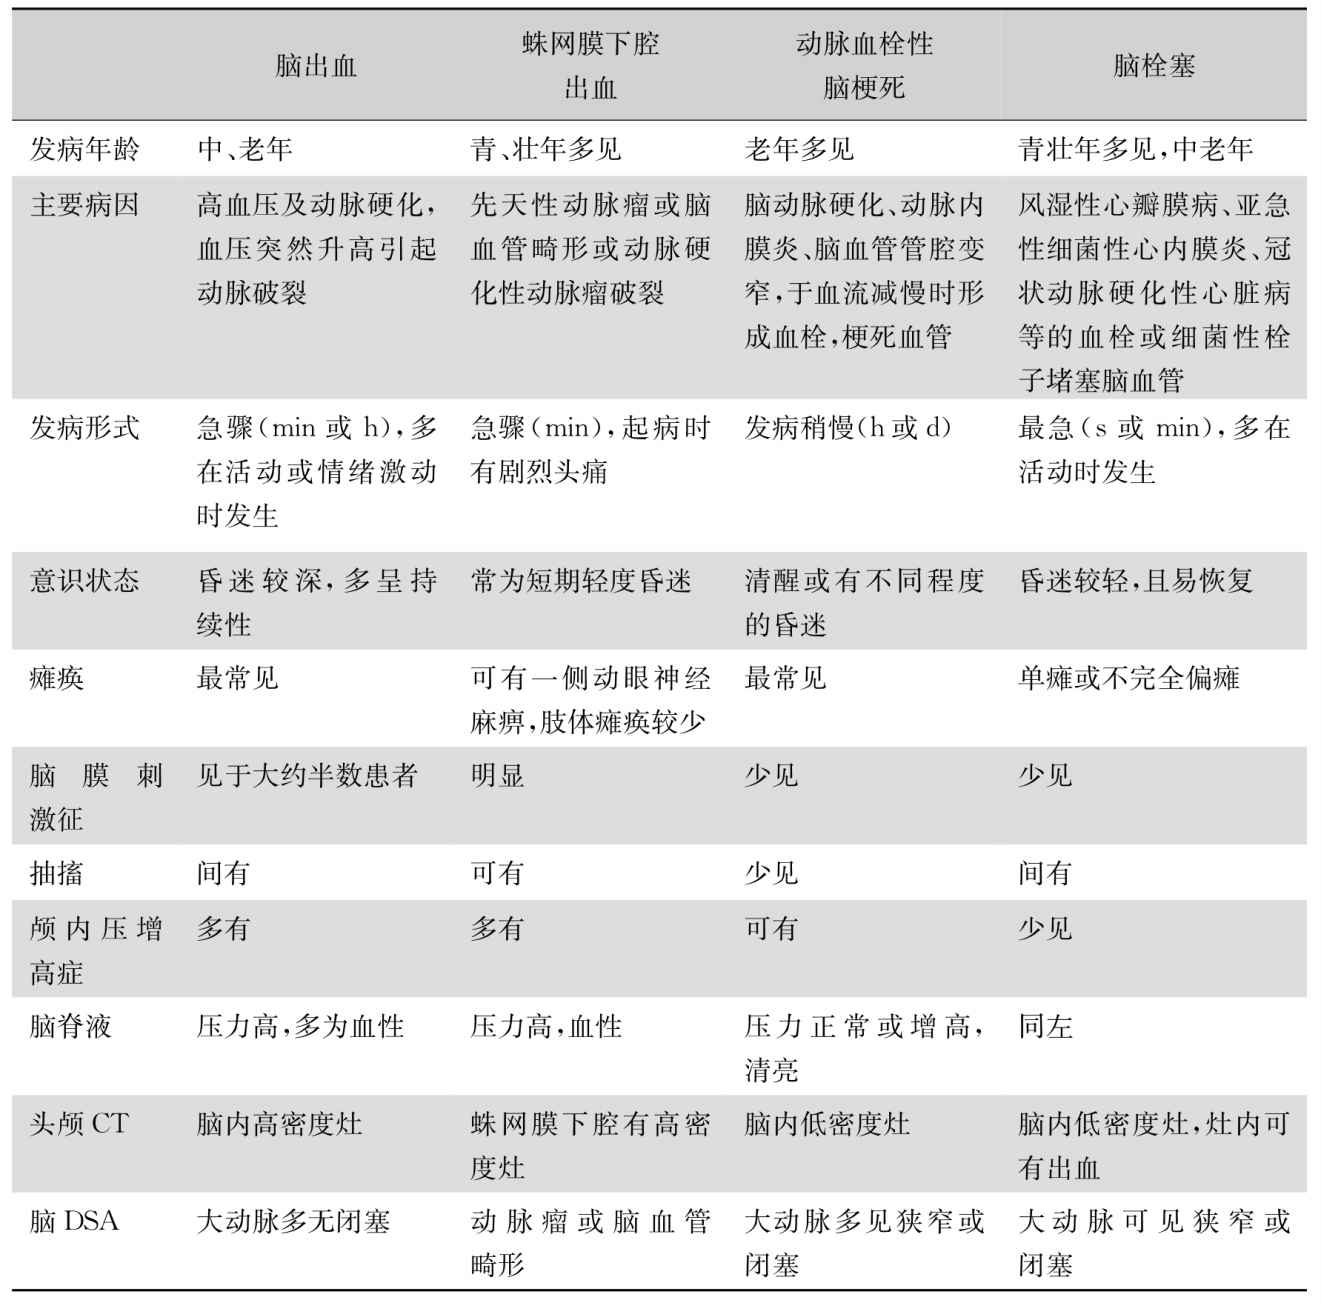
\includegraphics[width=5.9375in,height=5.85417in]{./images/Image00310.jpg}
\end{table}

\subsubsection{二、蛛网膜下腔出血}

蛛网膜下腔出血包括原发性与继发性蛛网膜下腔出血,前者是指位于脑表面的血管破裂出血进入蛛网膜下腔,年轻者多由颅底动脉瘤破裂或脑血管畸形出血所引起,年老者多与动脉硬化性动脉瘤破裂出血有关。后者是继发于脑实质出血(大脑半球、脑干或小脑出血)、颅脑损伤、脑肿瘤出血等破入蛛网膜下腔所致。本节所指的蛛网膜下腔出血即原发性蛛网膜下腔出血。

意识障碍是蛛网膜下腔出血常见而重要的症状。典型表现是突发性头痛、呕吐、意识障碍,后者以短暂而轻度昏迷为其特点,系大量血液进入蛛网膜下腔刺激脑膜及急性脑血管痉挛所致;进行性意识障碍、昏迷提示迟发性脑血管痉挛,常发生于蛛网膜下腔出血后一周左右,多伴有偏瘫或四肢瘫或癫痫发作;突然头痛、呼吸停止、昏迷提示枕骨大孔疝形成,常见于颅底动脉瘤再破裂出血,病情危重。继发性蛛网膜下腔出血的症状取决于原发病的状况,除可以出现意识障碍、昏迷外,还有明显的原发病症状和局部体征。预后亦与原发病的病情相关。

体检颈项强硬,Kernig征阳性,继发性蛛网膜下腔出血尚有原发病的症状和局部体征。头颅CT显示蛛网膜下腔有高密度影像学改变,可以确诊;腰穿脑脊液压力增高,均匀血性,在CT问世之后已不属确诊的必检项目。

\subsubsection{三、脑梗死}

脑梗死包括动脉粥样硬化性脑梗死和血栓性脑梗死(脑栓塞),前者是指在脑动脉粥样硬化等动脉壁病变的基础上形成管腔内血栓,造成该动脉供血区血流中断,局部脑组织发生缺血缺氧、坏死。脑栓塞是指脑动脉管壁上的粥样硬化斑块或心源性血栓脱落后引起的脑动脉栓塞。

意识障碍是脑梗死的主要症状之一,其发生与梗死灶的部位、大小和数量有关。

\paragraph{(一)基底动脉尖闭塞}

突出症状是昏睡或昏迷,多数患者昏迷持续的时间较短,脑神经损害可表现为单侧或双侧动眼神经麻痹,肢体瘫痪呈不完全性,可偏瘫或四肢瘫。

\paragraph{(二)基底动脉主干闭塞}

常引起广泛的脑桥梗死,表现为双眼不能内、外活动,不能言语、吞咽,四肢完全性瘫痪,大、小便潴留,但意识存在,患者可借助眼球上、下活动表达其意思,容易与昏迷混淆。

\paragraph{(三)急性颈内动脉闭塞}

急性颈内动脉闭塞如侧支循环代偿不良,可引起TIA发作或大片脑梗死,临床表现的严重程度不等,轻者对侧轻单瘫、轻偏瘫、同向偏盲,重者可完全性偏瘫、偏身感觉障碍、失语、失认,甚至嗜睡、昏迷。后者的发生与梗死灶的大小直接相关,多在发病后数小时开始,呈进行性加重。

\paragraph{(四)急性大脑中动脉主干闭塞}

可迅速出现意识障碍、对侧肢体完全性偏瘫;意识障碍以嗜睡开始,逐渐加重,数小时至数天可因进行性广泛性脑水肿、脑内高压发展至昏迷。多数病例在数天内死亡。

有些风湿性心脏病、多发性脑动脉炎或高血压动脉粥样硬化患者,临床上出现急性双侧性大脑半球损害的症状,轻者表现为四肢轻瘫,言语障碍;重者四肢瘫痪明显,意识障碍,轻者昏睡,重者昏迷,并出现假性延髓麻痹。首次发病者多数预后较好,但复发率高。头颅CT显示双侧大脑半球急性梗死灶,病灶多,但梗死体积不大。临床表现因病灶的多寡、大小不同而异,昏迷的发生可能与双侧大脑半球水肿有关(影响上行网状结构向皮层的投射)。

脑梗死的头颅CT(发病24小时后)可发现低密度病灶;MRI(发病6~12小时后)可显示T1低信号、T2高信号的梗死灶,并能发现脑干、小脑(CT不能显示的)小病灶。MRI弥散加权成像(DWI)和灌注加权成像(PWI)可发现更早期(20~30分钟)的缺血病灶,对溶栓治疗有指导价值。

脑梗死的诊断主要依靠临床表现和神经放射学检查。

\subsubsection{四、其他脑血管疾病}

高血压脑病及颅内静脉窦血栓形成等,均可发生不同程度的意识障碍。

\paragraph{(一)高血压脑病}

高血压脑病是指因急性肾炎、妊高征或恶性高血压等原因引起的血压骤然急剧升高所致的一种短暂性急性全面脑功能障碍综合征,一般血压突升至180/
120mmHg时即可发病,其机制至今尚不清楚。病理改变主要是广泛性脑水肿、脑小动脉壁纤维素样坏死、点状淤血或大量出血。主要临床表现为头痛、呕吐、黑蒙、烦躁、意识模糊、嗜睡、视物模糊和癫痫发作,如血压控制良好,症状可在数分钟至数日缓解,否则可导致昏迷甚至死亡。

\paragraph{(二)颅内静脉窦血栓形成}

是一组由多种病因引起的脑静脉系统血管病,临床症状因病变部位、病因不同而异。常见的病变部位为乙状窦、上矢状窦、直窦和大脑静脉等部位血栓形成;病因为外伤、妊娠期或产褥期的血高凝状态、感染、肿瘤转移、血液病等。临床表现为头痛、呕吐等颅内压增高症状,严重时可出现意识模糊、嗜睡甚至昏迷。可有抽搐、脑神经损害和双下肢无力或瘫痪等局限性体征。

头颅CT和MRI可见窦旁出血、水肿、脑室变小、窦旁静脉扩张。脑血管造影可见血栓形成的静脉窦和引流静脉不显影。

\protect\hypertarget{text00377.html}{}{}

\subsection{164.3 脑占位性疾病}

脑肿瘤引起的昏迷往往是疾病的后期。下述几种情况有导致昏迷的可能:①颅内压逐渐增高,继发脑疝;②肿瘤内血管破裂(脑瘤性卒中);③脑室系统及其附近的肿瘤突然闭塞脑脊液的循环通路,引起昏迷。典型的临床特征是进行性头痛、呕吐与眼底水肿(参见第155节)。

脑脓肿引起颅内压增高时,常有嗜睡、昏睡等意识障碍,及至脑疝形成时可发生昏迷;或者是脓肿穿破,引起急性脑膜炎时也发生昏迷,因此昏迷常是脑脓肿的垂危征象。耳源性脑脓肿所致的昏迷,与化脓性脑膜炎(尤其是耳源性者)颇难鉴别。如在昏迷前有局限性体征(颞叶或小脑损害征),则脑脓肿的可能性大。此外,脑脓肿患者的脉搏规则、充实和缓慢;脑膜炎患者的脉搏往往细速而不规则。脑脓肿的脑脊液改变是细胞轻度增加,糖与氯化物正常;脑膜炎则细胞显著增多,糖与氯化物含量降低。

\protect\hypertarget{text00378.html}{}{}

\subsection{164.4 闭合性颅脑损伤}

颅脑外伤是发生意识障碍的常见原因之一。据国外某组1167例昏迷病因的分析,由于外伤引起者为152例(13\%),居第二位。本文仅述及闭合性颅脑损伤所致的昏迷。通常将闭合性颅脑损伤简单分为原发性脑损伤与继发性脑病变两类,前者如脑震荡、脑挫裂伤,后者如脑水肿、颅内血肿、脑疝等。同一患者可存在多种不同的损伤。昏迷的程度和持续的时间,一般与损伤的轻重相一致。

\subsubsection{一、脑震荡}

头部外伤后立即发生的中枢神经系统一时性功能障碍,谓之脑震荡。脑震荡可单独发生,或合并其他类型的颅脑损伤。伤者在受伤后立即出现意识障碍,其程度可为一时的神志恍惚乃至意识完全丧失;其持续时间仅数秒至数分钟,一般不超过半小时。伤者面色苍白,双侧瞳孔散大或缩小,对光反射消失,肌张力降低,脉慢而弱,呼吸缓慢,全身出汗,历时数秒钟、数分钟,或迟至20~30分钟内恢复。几乎所有的伤者于清醒后对所发生的情况都不能回忆,称为逆行性遗忘,这是本病的特征之一。伤者也往往对醒后的一段时间发生遗忘,称为顺行性遗忘。此外,伤者多有头痛、头晕、恶心、怕光、出汗、注意力涣散、记忆力减退、失眠等,持续数天渐消失。如此等症状长时间(3个月以上)继续存在,即构成临床上的脑外伤后遗症。头颅CT
或MRI无阳性发现。

诊断脑震荡的依据是:①头部外伤后即时出现短暂的意识障碍及近事遗忘;②除上述瞳孔与肌张力改变之外,神经系统检查一般无明显异常;③脑脊液检查正常;④头颅CT或MRI无阳性发现。脑震荡主要需与脑挫裂伤以及颅内血肿相鉴别(详见后述)。

\subsubsection{二、脑挫裂伤}

脑挫裂伤是指头部外伤后脑组织发生器质性损伤。受伤后伤者即时出现不同程度的昏迷,从嗜睡状态直至深度昏迷,持续半小时至数小时、数天、数周或数月以上,偶尔可达数年。脑挫裂伤后继发脑水肿,临床表现有颅内压增高征象,如剧烈头痛、呕吐、血压升高及脉搏减慢等。如伤者出现躁动不安而意识障碍随之加深时,应警惕脑疝形成的可能;如伤者出现躁动而意识障碍的程度前后相似,则可能属于创伤疼痛或尿潴留等身体不适,也可能是伤情趋向好转的现象。由于脑损伤的部位不同而出现各种神经系统定位体征,如肢体瘫痪、脑神经瘫痪、感觉障碍、失语、癫痫样抽搐等。此外,在恢复期间的头痛、头晕、出汗、恶心、记忆力减退、失眠等症状也较脑震荡显著。

脑挫裂伤不同于脑震荡的要点是:①昏迷时间较长和程度较重;②神经系统检查往往有定位体征;③脑脊液压力升高,可混有血液;④头颅CT或MRI可见点片状出血。脑挫裂伤与颅内血肿的区别在于:①前者在伤后立即出现症状和体征,而后者的症状和体征是逐渐发展的,且在昏迷期间可有中间清醒或好转期;②伤后即刻出现单瘫或偏瘫而无对侧瞳孔散大者多为脑挫裂伤,如伤后一段时间才出现偏瘫而对侧瞳孔散大者多为颅内血肿;③脑挫裂伤的头颅CT或MRI见点片状出血,后者见颅内血肿。但两者常并存。

\subsubsection{三、外伤性颅内血肿}

颅脑损伤后出现下列情况时,应高度怀疑颅内血肿的可能:

\paragraph{1.意识改变}

①伤后昏迷转为清醒或者意识好转,然后再度昏迷;②伤后清醒,以后转为昏迷;③伤后持续昏迷且进行性加深。

\paragraph{2.急性颅内压增高}

伤后头痛持续和加剧,或伴有呕吐而意识障碍又呈进行性加深。

\paragraph{3.脑疝形成}

伤后逐渐出现一侧瞳孔扩大而对侧肢体呈现进行性瘫痪(或有锥体束征),是小脑幕切迹疝(颞叶钩回疝)的表现。脑疝的出现常是颅内血肿较为后期的表现。

颅内血肿按其部位可分为硬脑膜外血肿、硬脑膜下血肿和脑实质内血肿,分述于下:

\paragraph{(一)硬脑膜外血肿}

是指出血积聚于颅骨与硬脑膜之间的血肿。大多由于颅骨骨折使脑膜中动脉(或静脉)破裂所致;次为静脉窦破裂;有时是板障静脉或导血管破裂出血所引起。典型表现是伤后立即有短暂昏迷(由于脑震荡或脑挫裂伤所致),继而意识清醒或好转(中间清醒期),旋又进入再次昏迷(由于颅内血肿形成)。但此种昏迷→清醒→昏迷的典型病例并不多见,约占30\%。伤者有颅内压增高,清醒时感到头痛、恶心、呕吐。多有烦躁不安、意识进行性障碍、血压升高、脉缓而充实等,并逐渐出现伤侧瞳孔散大、对光反射迟钝或消失(动眼神经受压),对侧肢体瘫痪或有锥体束征(血肿压迫局部大脑皮质或颞叶钩回压迫大脑脚)。

诊断除依靠上述临床表现外,在伤者病情许可的情况下,争取早期作头颅CT扫描,在颅骨内面和脑表面之间出现凸透镜形或弓形高密度影,并且周边可见水肿带及脑室受压和中线结构移位的影像学改变。若病情危急,来不及CT检查或没有CT设备时,也可直接钻颅探查,以争取时间抢救伤者的生命。

\paragraph{(二)硬脑膜下血肿}

是由于颅脑损伤后大脑表面的浅静脉或皮质小动脉破裂出血,血液积聚于硬脑膜下间隙所致。按病程发展分为急性、亚急性与慢性三种,急性者在3天之内,亚急性者3天~3周,慢性者3周以上。急性与亚急性在病理上并无明显区别。

\subparagraph{1.急性与亚急性硬脑膜下血肿}

伤者的伤势较重,多合并广泛严重的脑挫裂伤,常为双侧性。受伤后持续昏迷,进行性加重,少数有中间清醒期。主要表现是原发性脑损伤及继发性脑受压的混合改变。临床上急性颅内压增高、生命体征改变以及颞叶钩回疝出现早,进展快。伤后早期常有一侧肢体表现为不完全性瘫痪,并呈进行性加重,还可有部分性癫痫发作。头颅CT扫描绝大多数患者在颅板下方出现新月形高密度区,范围广泛时可为双凸型。部分患者可高、低密度同时并存,有时高密度区局限于血肿下部而出现液平面,系由部分溶血后血红蛋白释出下沉所致,血肿周围可见水肿带;病侧脑组织可见受压水肿移位。根据头颅CT检查诊断并不困难,如情况危急可行钻颅探查。

\subparagraph{2.慢性硬脑膜下血肿}

多因头部受到较轻的外伤所引起,常为大脑凸面表浅静脉缓慢出血的结果。早期症状较轻或无明显症状。约经3~4周后,血肿逐渐增大时始出现头痛、呕吐、嗜睡、视乳头水肿等颅内压增高症。意识也呈进行性障碍,也可出现脑受压的局灶体征或小脑幕切迹疝。若病程较长又无明确外伤史(由于外伤较轻或外伤距离发病时间太长致伤者不复记忆),临床易误诊为脑肿瘤。CT检查在紧贴颅骨内板下方可见双凸形或平凸形血肿影,其密度可因血肿期龄不同而有所差异,多数表现为密度降低,部分可为等密度或略高密度,侧脑室常常受压变形或消失。单侧病变中线结构向对侧移位,双侧时可无移位。强化可显示血肿包膜。MRI可显示独特的T1加权、T2加权均表现为高信号,对本病的诊断有重要价值。

\paragraph{(三)脑实质内血肿}

急性脑实质内血肿多在严重脑挫裂伤的基础上形成,且往往与急性硬脑膜下血肿并存,故颇难作出单独的诊断。

慢性脑实质内血肿与慢性硬脑膜下血肿的症状相似,但前者的定位体征有时较后者明显。

\protect\hypertarget{text00379.html}{}{}

\subsection{164.5 颅内压增高综合征与脑疝形成}

正常情况下,脑和脑膜的体积与颅腔容积之间的差别约为10\%(8\%~10\%),颅腔内通过血液循环和脑脊液循环起调节作用,并维持适当的颅内压力。侧卧位腰椎穿刺测量脑脊液压力时,成人正常值为70~180mmH\textsubscript{2}
O(20~50滴/分)。由于某些病变引起颅内容物体积增加或颅腔容积缩小,均可产生颅内压增高。颅内压增高的主要病理基础是脑水肿(包括脑肿胀),其原因是:①脑小血管壁或血脑屏障的通透性增加;②脑组织渗透压增高或血液渗透压减低;③脑血液循环障碍,表现为脑静脉血流淤滞和动脉血流减少;④脑脊液的生成、吸收障碍和循环梗阻。这四者互为因果,造成恶性循环,导致颅内压力不断增高。颅内压增高在临床上有其特殊表现,称为颅内压增高综合征。颅内压增高的严重性是脑疝形成。

颅内压增高通常分为急性与慢性两种。慢性者由于机体的代偿作用,可在较长时间内不出现危险,但因某些因素的促发可突变为急性颅内压增高,甚至发生脑疝。

\subsubsection{一、疾病种类}

引起颅内压增高的疾病种类很多,大致分为下列几项:

\paragraph{1.颅内或颅外急性或慢性感染}

如脑膜炎、脑炎、脑蛛网膜炎、中毒性肺炎或中毒性菌痢、败血症,以及其他原因所致的感染中毒性脑病。

\paragraph{2.脑血液循环障碍所致的疾病}

如脑出血、蛛网膜下腔出血、脑动脉血栓形成性脑梗死、脑栓塞、高血压脑病、颅内静脉窦血栓形成等。

\paragraph{3.颅脑损伤}

如脑震荡、脑挫裂伤、颅内血肿、脑部手术伤等。

\paragraph{4.颅内占位性疾病}

如脑肿瘤、脑脓肿、脑寄生虫病等。

\paragraph{5.颅脑先天性畸形}

如先天性脑积水、颅狭窄症、小头畸形、颅骨发育异常等。

\paragraph{6.各种原因引起的缺氧}

如窒息、循环骤停、癫痫持续状态等。

\paragraph{7.中毒}

工业毒物、农药、药物、食物等中毒。

\paragraph{8.其他}

如尿毒症、肝性脑病、血小板减少性紫癜、脑型白血病、再生障碍性贫血、真性红细胞增多症、肾上腺皮质功能亢进症或减退症、甲状旁腺功能减退症、急性水中毒、中暑、妊娠中毒症、严重的输血或输液反应、放射性脑病等。

\subsubsection{二、临床表现}

颅内压增高症的临床表现主要有下述几方面:

\paragraph{(一)一般症状}

常见者为头痛、头晕、眩晕、呕吐、耳鸣等。头痛是由于颅内痛敏结构(结膜、血管、神经)受刺激、牵拉或压迫所致。头痛的性质可为钝痛、胀痛、牵扯痛,部位多为全头部。头痛以清晨最剧烈,有时下半夜痛醒。凡能促使颅内压增高的动作如摇头、弯身、咳嗽、用力排便等,均可导致头痛加剧。颅内压逐渐增高时,头痛程度也随之增加。患者还可有单侧或双侧展神经轻瘫,这是由于该神经在颅底行程较长、易遭受损害所致,并无定位价值。

\paragraph{(二)意识障碍及精神症状}

早期患者表现为呆滞、淡漠、嗜睡或神志恍惚。颅内压急剧增高乃至发生脑疝时,患者的意识障碍急转直下,进入昏迷,可有兴奋、躁动或癫痫样抽搐,再进而呈深昏迷。慢性颅内压力增高者可产生脑积水,继发脑萎缩,出现行为异常、痴呆等。

\paragraph{(三)生命体征变化}

颅内压增高使脑组织缺氧,机体发挥代偿作用使血压升高,脉慢而洪大,呼吸深慢。随着颅内压力的继续增高,此三种变化可更明显,收缩压可上升至200mmHg,心率可减慢至40次/分,呼吸可变得不规则,或出现抽泣样呼吸、间歇呼吸等。后期则因延髓功能衰竭而致血压下降、脉速而弱,呼吸停止。

\paragraph{(四)眼底及瞳孔改变}

颅内压力增高的重要体征是眼底改变。由于颅内压增高使视神经鞘内的脑脊液压增高,导致视神经的组织压力也增高,轴浆流动停滞,眼静脉回流也受阻,因而发生静脉充血及视乳头水肿。急性而严重的颅内压增高可于三天甚至数小时内出现视乳头水肿,后者成为急性颅压增高的佐证;慢性颅压增高者多在数周内出现视乳头水肿。瞳孔改变在颅内压增高尤其是脑疝形成时最明显,且有诊断意义。丘脑下部单侧受累时,该侧瞳孔缩小;如双侧受累则表现为双侧瞳孔缩小。倘若双侧瞳孔对光反射消失,说明中脑已有广泛损害。小脑幕切迹疝压迫该侧动眼神经时,瞳孔可先缩小,短时后扩大。若病灶将对侧脑组织推移压向对侧骨壁,则病灶对侧的瞳孔先扩大。

\paragraph{(五)癫痫样抽搐}

因脑细胞缺血缺氧所致。

\paragraph{(六)锥体束受累征}

颅内压增高可引起大脑皮质运动区受损,或继发脑干受损,出现锥体束受损征象或轻偏瘫。小脑幕切迹疝可引起偏瘫或四肢瘫。

\paragraph{(七)颅骨改变}

慢性颅内压增高时才有颅骨改变。X线平片可见蝶鞍骨质吸收以及蝶鞍扩大、脑回压迹增加等。头颅CT或MRI见脑肿胀、脑干及(或)脑室可受压,中线移位。

颅内压力增高时,腰椎穿刺可促发脑疝,通常列为禁忌。如因诊断或鉴别诊断的需要,应极为谨慎地进行,使用小号腰穿针,尽可能慢放、少放脑脊液。

某些病变(如颅脑损伤)可引起继发的低颅压综合征,表现为剧烈头痛、眩晕、呕吐,甚至颈强硬或发作性昏睡等,易误诊为颅内压增高症。两者的头痛有所不同:低颅压时头痛在头高位时加重,头低位时减轻,饮水后或静脉滴注低渗溶液后头痛也得以减轻;高颅压时则相反。低颅压时眼底视乳头无水肿现象,颅骨X线平片也无改变。头颅CT或MRI未见异常改变。

\subsubsection{三、脑疝形成}

颅腔内某部分脑组织向压力较低的部位发生移位现象,称为脑疝。导致脑疝形成的主要因素是颅内压力增高,但后者并非引起脑疝的唯一条件,只有颅内压严重增高或急剧增高时才会发生脑疝。此外,也可因某些因素(如腰椎穿刺)的促发而引起脑疝。脑疝的危险性不仅是疝入的脑组织发生淤血、出血、水肿和软化,以及某一脑池被堵塞;更重要的是疝入物压迫附近的脑组织(最常是脑干)和血管、脑脊液通道等,引起继发的脑血液和脑脊液循环严重障碍,以及生命中枢功能障碍,并形成恶性循环。脑疝有多种,常见的是小脑幕切迹疝和枕骨大孔疝两种。

\paragraph{(一)小脑幕切迹疝(颞叶钩回疝)}

一侧颞叶钩回向内下方移位,嵌顿于小脑幕切迹,称为小脑幕切迹疝。最常见的是由于小脑幕上病变所引起,如病变为占位性,则其常见的部位是颞叶与内囊。小脑幕切迹疝的主要表现是:①头痛显著增剧,使患者难以忍受;②意识障碍逐渐加重,开始时患者嗜睡或躁动不安,进一步陷于浅昏迷,再进而为深昏迷,意识变化主要是由于中脑上行性网状激活系统受损所致;③疝侧瞳孔散大是诊断小脑幕切迹疝的重要指征,因脑疝对该侧动眼神经的压迫引起疝侧瞳孔散大,对光反射消失(开始时瞳孔可先缩小,对光反射迟钝),极少数病例是对侧瞳孔先散大,晚期由于双侧动眼神经均受压,而致双侧瞳孔散大;④疝侧的大脑脚被压,而致对侧肢体瘫痪或出现锥体束征,偶尔瘫痪是在病灶同侧肢体,乃因脑疝推移中脑,使对侧大脑脚压于小脑幕切迹或岩骨嵴上之故;⑤生命体征改变已如前述,脑疝初期体温升高,极期体温更高,后期则体温下降,低于正常温度;⑥部分患者出现颈硬,某些患者则因中脑受损出现去大脑强直现象,少数病例发生失明,可能是大脑后动脉受压使枕叶软化所致;⑦头颅CT或MRI可见脑肿胀、脑干受压、移位。

\paragraph{(二)枕骨大孔疝(小脑扁桃体疝)}

小脑扁桃体下降于枕骨大孔内或椎管内,称为枕骨大孔疝,主要由于小脑幕下病变所引起,而小脑幕上病变也可引起。枕骨大孔疝可单独出现或继发于小脑幕切迹疝,其严重性在于延髓受压。最早的症状是颈部有阻力或颈项强硬、强迫头位,是由于局部神经受牵扯所表现的防御反射。最主要的症状是呼吸改变,患者的呼吸常突然停止。双侧瞳孔散大且对光反射消失,乃由于动眼神经核受损所致。慢性枕骨大孔疝大多表现为颈痛、颈硬,而无其他症状。

颅内压增高的患者出现下列征象时,有助于脑疝的早期诊断:①头痛突然显著加剧,常是脑疝发生的前奏;②意识障碍加重,尤其是躁动不安,预示脑疝的来临;③瞳孔改变,开始时双侧瞳孔可缩小,或忽大忽小,继则双侧瞳孔不等大;④患者出现颈痛或颈硬或有强迫头位时,应警惕枕骨大孔疝的发生;⑤呼吸骤停,是枕骨大孔疝发生的征兆;⑥临床表现为颅内压增高症,但腰椎穿刺时脑脊液压力不高,应怀疑有枕骨大孔疝的存在,可能是从颅腔通向椎管的道路有梗阻,腰椎穿刺所测得的压力未能真正反映颅内压力;⑦头颅MRI矢状面可见小脑扁桃体下降于枕骨大孔内或椎管内,嵌顿于脑干、延髓。当怀疑患者有脑疝时,腰椎穿刺应为禁忌。

小脑幕切迹疝与枕骨大孔疝的鉴别是:①前者的意识障碍较后者出现为早;②后者以呼吸变化为主征;③前者以一侧瞳孔散大为诊断的主要依据,后者可见双侧瞳孔散大;④早期出现颈痛、颈硬多见于枕骨大孔疝;⑤前者多伴有脑疝的对侧肢体瘫痪,后者较少见。

\protect\hypertarget{text00380.html}{}{}

\subsection{164.6 癫痫}

意识障碍是癫痫大发作、癫痫失神发作(典型和非典型)、复杂部分性发作以及癫痫持续状态的主征。各型癫痫的诊断和鉴别诊断参见第51章。

\protect\hypertarget{text00381.html}{}{}

\section{参考文献}

1.Dyken PR.Neuroprogressive disease of post-infectious origin:a review
of a resurging subacute sclerosing panencephalitis(SSPE).Ment Retard
Dev Disabil Res Rev,2001,7(3):217-225

2.Ferenci P,et al.Hepatic
encephalopathy-definition,nomenclature,diagnosis,and
quantification:final report of the working party at the 11th World
Congresses of Gastroenterology,Vienna,1998.Hepatology,2002,35
(3):716-721

3.Yared Z,Chiasson JL.Ketoacidosis and the hyperosmolar hyperglycemic
state in adult diabetic patients.Diagnosis and treatment.Minerva
Med,2003,94(6):409-418

4.Moritz ML,Ayus JC.New aspects in the pathogenesis,prevention,and
treatment of hyponatremic encephalopathy in children.Pediatr
Nephrol,2010,25(7):1225-1238

5.Sungur M,Güven M.Intensive care management of organophosphate
insecticide poisoning.Crit Care,2001,5 (4):211-215

6.Mendelow AD,et al.Early surgery versus initial conservative treatment
in patients with spontaneous supratentorial intracerebral haematomas in
the International Surgical Trial in Intracerebral Haemorrhage
(STICH):a randomised trial.Lancet,2005,365(9457):387-397

\protect\hypertarget{text00382.html}{}{}

